\documentclass[UTF8,fontset=fandol,11pt,openany]{ctexbook}
\usepackage[a4paper,margin=25mm,headheight=15pt]{geometry}
\usepackage{graphicx}
\usepackage{booktabs}
\usepackage{longtable}
\usepackage{tabularx}
\usepackage{array}
\usepackage{enumitem}
\usepackage{listings}
\usepackage[most]{tcolorbox}
\usepackage{fancyhdr}
\usepackage{microtype}
\usepackage{xcolor}
\usepackage{hyperref}

\definecolor{HandbookGreen}{HTML}{176B5B}
\definecolor{HandbookOrange}{HTML}{C4682D}
\definecolor{HandbookInk}{HTML}{202725}
\definecolor{HandbookGray}{HTML}{F2F4F3}
\hypersetup{colorlinks=true,linkcolor=HandbookGreen,urlcolor=HandbookOrange}
\graphicspath{{./}}
\setlength{\parindent}{2em}
\setlength{\parskip}{0.35em}
\setlength{\emergencystretch}{4em}
\tolerance=2500
\sloppy
\setlist{nosep,leftmargin=2em}
\renewcommand{\arraystretch}{1.25}

\pagestyle{fancy}
\fancyhf{}
\fancyhead[L]{ECom Review Intelligence Agent}
\fancyhead[R]{\leftmark}
\fancyfoot[C]{\thepage}

\lstset{
  basicstyle=\ttfamily\small,
  backgroundcolor=\color{HandbookGray},
  frame=single,
  rulecolor=\color{HandbookGray},
  breaklines=true,
  columns=fullflexible,
  showstringspaces=false
}

\newtcolorbox{factbox}{title=已有证据支持的事实,colback=green!4,colframe=HandbookGreen}
\newtcolorbox{inferencebox}{title=基于证据的推断,colback=blue!3,colframe=blue!45!black}
\newtcolorbox{advicebox}{title=建议,colback=orange!4,colframe=HandbookOrange}
\newtcolorbox{boundarybox}{title=尚待验证或适用边界,colback=red!3,colframe=red!55!black}
\newtcolorbox{beginnerbox}{title=初学者提示,colback=HandbookGray,colframe=gray!60!black}
\newtcolorbox{interviewbox}{title=面试提示,colback=yellow!5,colframe=HandbookOrange}

\newcommand{\filelink}[1]{{\small\nolinkurl{#1}}}
\newcommand{\statuspassed}{\textcolor{HandbookGreen}{\textbf{PASSED}}}
\newcommand{\statusprogress}{\textcolor{HandbookOrange}{\textbf{\scriptsize IN\_PROGRESS}}}


\title{ECom Review Intelligence Agent\\项目学习与面试手册}
\author{项目公开学习版}
\date{2026 年 8 月}

\begin{document}
\frontmatter
\maketitle
\chapter*{公开边界说明}
本文档只使用可公开的聚合信息和仓库相对路径，不包含原始评论、真实商品或证据标识、密钥及私有求职材料。
\tableofcontents

\mainmatter
\chapter{项目概览与阅读指南}

\section{先用一句话理解项目}

ECom Review Intelligence Agent 是一个面向 B 端电商运营的评论证据决策原型。你可以把它理解成一位“会查评论、会整理证据、但不会替运营拍板”的助手：运营提出一个商品问题，系统返回可回查的评论证据，帮助单品诊断、商品比较和问题分流。它不是面向 C 端消费者的购物推荐助手，也不会根据评论自动推断真实缺陷率、销量或利润。

\begin{beginnerbox}
先记住项目的完整故事：P0、P1 先把数据用对；P2 决定先研究哪个商品范围；P3 规定“什么算一个问题”；P4 让人能快速找到原始证据；P5 比较不同查找方法；P6 才让模型按步骤调用工具；P7 检查目标运营人员是否真的愿意使用。后面每一步都在解决前一步留下的具体问题。
\end{beginnerbox}

\begin{beginnerbox}
这里的“证据”不是指系统已经证明某个商品真的存在质量缺陷，而是指：系统给出的判断能够返回到本地、冻结数据中的对应评论记录，供运营人员继续复核。评论信号是后续调查的输入，不是现实世界结论。
\end{beginnerbox}

\section{开始前需要知道的状态}

\begin{factbox}
仓库当前可验证状态为 P0--P6 \statuspassed；P7 为 \statusprogress。

合成浏览器流程和受控本地工程回归已有通过证据，但真人目标运营用户尚未完成结构化试用。因此，不能把这一阶段写成通过，也不能声称项目已经为企业降本增效。
\end{factbox}

阶段状态和放行条件以 \filelink{docs/master-plan.md} 为执行权威；当前状态摘要见 \filelink{docs/current-stage-status.md}；阶段学习、失败复盘与面试边界见 \filelink{docs/interview-casebook.md}。阶段报告位于 \filelink{docs/reports/}。这些都是仓库相对路径，不依赖某台电脑的目录结构。

\section{四类信息必须分开}

阅读本手册时，不要把“看起来合理”当成“已经证明”。正文使用以下四种信息类型。

\begin{factbox}
\textbf{事实：}已有仓库产物、测试、审计或阶段报告支持。例如，P6 的冻结案例工程门已经通过。这类表述仍然受数据快照、案例范围和配置版本限制。
\end{factbox}

\begin{inferencebox}
\textbf{推断：}从已有事实出发得到的合理解释。例如，评论证据工作台可能减少重复查找和整理评论的机械操作。它有理由成立，但在真人任务试用前还不是业务结果。
\end{inferencebox}

\begin{advicebox}
\textbf{建议：}下一步应做的产品或工程动作。例如，先让目标运营用户完成同一组手工任务和工作台任务，再比较完成时间与证据复核情况。建议不是已经完成的工作。
\end{advicebox}

\begin{boundarybox}
\textbf{待验证：}当前证据不足以确认的信息，包括真实需求频率、用户采纳率、付费意愿、实际节省时间、决策质量改善和生产环境可靠性。证据不足不等于这些结论一定错误，只表示现在不能声称它们成立。
\end{boundarybox}

\section{先理解 P0 与 P1：数据地基}

第一次阅读时，可以把 P0 和 P1 当成一个学习单元，连续回答两个问题：

\begin{enumerate}
\item P0：这批数据能不能放心用？
\item P1：之后的分析是不是一直在用同一版数据？
\end{enumerate}

举个运营例子：你今天发现某类商品的“漏水”反馈比较集中。下周重新运行时，如果换了一份文件，结果变化可能只是数据换了，并不代表商品真的变好或变坏。P0 先检查数据来源、字段和使用边界；P1 再给本次输入做版本记录。这样后面的结论才有机会比较和复盘。

\begin{beginnerbox}
P0/P1 的业务价值不是立刻生成销售结论，而是避免“做了很久才发现数据不能用”以及“每次运行都不知道自己用了哪批数据”。技术名词先不用背，等读到对应阶段时再看术语卡。
\end{beginnerbox}

\section{初学者术语表}

\begin{longtable}{>{\raggedright\arraybackslash}p{0.18\textwidth}>{\raggedright\arraybackslash}p{0.72\textwidth}}
\toprule
术语 & 通俗解释 \\
\midrule
\endfirsthead
\toprule
术语 & 通俗解释 \\
\midrule
\endhead
B 端 & 企业或团队内部使用的工具。本项目的主用户是产品或类目运营。 \\
C 端 & 普通消费者直接使用的产品。本项目不做消费者选购助手。 \\
SKU & 一个具体可区分的商品单元。手册中的“单品诊断”可以先理解为针对一个指定商品查找评论证据。 \\
VOC & Voice of Customer，即“客户之声”。在本项目中，它指从评论中整理出来的体验维度和问题信号。 \\
Agent & 能根据请求选择既定步骤和工具的软件流程。这里的 Agent 不能任意执行代码或查询，模型只提出受约束的计划和表达。读到 P6 再深入理解。 \\
确定性工具 & 输入相同时按照固定规则查询和计算的本地代码，例如商品解析、证据检索和引用校验。 \\
Verifier & 验证器。它不相信模型“说自己正确”，而是逐项核对商品范围、证据强度、引用和结果状态。 \\
Gate & 阶段闸门或放行条件。先把它理解成“这一关的检查清单”；只有规定的输入、产出和阻断指标都满足，阶段才可以标为通过。 \\
Lineage & 数据血缘。先把它理解成“结果是从哪里来的记录”：哪一批数据、哪套规则和哪份代码。 \\
Silver 标签 & 由冻结规则自动构造的期望结果，适合回归测试，但不是人工双审得到的 gold 标签。 \\
失败关闭 & 条件不满足时停止正常输出并返回明确错误或“证据不足”，而不是猜测一个看似完整的答案。 \\
\bottomrule
\end{longtable}

\section{推荐阅读顺序}

本手册采用一条按阶段推进的项目故事。第一次阅读请先读“项目为什么值得做”，然后依次读 P0--P7；P0/P1 作为“数据地基”连续理解，Agent 知识会在 P4--P6 的真实开发顺序中出现，而不是作为与证据系统分离的课程。

\begin{tabularx}{0.94\linewidth}{>{\raggedright\arraybackslash}p{0.18\textwidth}X}
\toprule
读者目标 & 建议路径 \\
\midrule
第一次接触项目 & 先读“为什么做”，再读 P0--P7，理解每一步在保护什么结论。 \\
完整学习工程 & 按 P0--P7 连续阅读；到 P6 时回看 P3--P5 的合同、工具与检索证据，理解模型为何不掌握最终事实。 \\
准备业务或产品面试 & 重点阅读用户、三个工作流、价值边界、阶段业务价值和真人验证缺口。 \\
准备技术面试 & 重点阅读数据血缘、确定性工具、Structured Output、Verifier、LangGraph、checkpoint 和评测失败复盘。 \\
准备简历 & 先确认当前状态和证据，再提炼“问题、行动、技术选择、可核实结果、边界”，不要只抄测试数字。 \\
\bottomrule
\end{tabularx}

\begin{advicebox}
基础较弱时，不需要先背框架名或哈希字符串。每读一个阶段，先回答三个问题：它要解决哪个运营问题？它留下了什么可以检查的结果？它还不能证明什么？能回答后，再学习对应技术会更稳固。
\end{advicebox}

\section{全书共同遵守的表达边界}

\begin{boundarybox}
本手册不得把自动化测试写成真人验收，不得把 silver 指标写成人工质量，不得把评论信号写成缺陷或因果事实，也不得把内部原型写成已上线企业 SaaS。公开材料只使用代码、合成夹具、聚合指标和经审查的结果；不展示原始评论、真实商品或证据标识、密钥和本地绝对路径。
\end{boundarybox}

\chapter{为什么做：业务起点与价值边界}

\section{先拆开动机、证据和假设}

“为什么做这个项目”不能只回答“电商很热门”，也不能把个人经历直接包装成市场需求。更可靠的起点是把三类信息分开。

\begin{factbox}
\textbf{本人确认的动机：}项目负责人以广州实习和后续求职为主要场景，希望同时展示 AI 产品、数据产品与 AI 应用、Agent 工程能力。由于当前实习位于运营中心，项目选择“运营如何从大量评论中形成可复核判断”作为主问题，而不是选择与个人经历脱节的通用聊天机器人。
\end{factbox}

\begin{inferencebox}
\textbf{有限的方向证据：}私有岗位样本中出现过 AI 产品、AI 应用、Agent、电商、跨境运营和供应链相关职责。这支持“该项目与部分目标岗位有交集”，但不能外推为广州完整招聘市场，也不能证明所有电商企业都有相同需求。私有岗位明细不属于公开手册证据。
\end{inferencebox}

\begin{boundarybox}
\textbf{待验证的产品假设：}产品或类目运营可能希望减少重复阅读评论的时间，并让单品诊断、竞品比较和问题分流返回可复核证据。需求强度、使用频率、现有替代流程、团队协作方式和付费意愿仍需访谈或工作流试用验证。
\end{boundarybox}

上述区分见 \filelink{docs/master-plan.md} 的“为什么做这个项目”和 \filelink{docs/interview-casebook.md} 的 Part 0。

\section{项目服务谁}

\subsection{B 端主用户与协作方}

\begin{factbox}
\textbf{主要用户}是耐用消费品品牌方或跨境电商团队中的产品、类目运营。产品、质量和客服团队是证据的协作消费者，但 MVP 不为四类角色分别建立四套独立产品。
\end{factbox}

只选择一个主用户有两个原因。第一，运营人员更直接面对商品范围、评论筛选和竞品比较；第二，单一主用户能控制 MVP 范围，使数据、工具和界面围绕同一工作流闭环。协作角色仍然可以使用运营整理后的证据，例如质量团队继续核查问题，客服团队更新知识内容。

\subsection{三个业务工作流}

\begin{enumerate}
  \item \textbf{单 SKU 体验诊断：}围绕一个指定商品和体验维度，整理支持、反对、冲突或证据不足的评论信号。
  \item \textbf{商品证据比较：}在两个到五个指定商品之间，按同一体验维度比较各自证据，而不是直接宣布“谁最好”。
  \item \textbf{问题信号分流：}根据冻结证据规则，整理哪些评论问题值得先核查。这里的优先级是调查顺序，不是缺陷严重度或财务损失排序。
\end{enumerate}

\begin{beginnerbox}
Excel 或 BI 擅长结构化汇总，普通聊天模型擅长开放表达。本项目关注的是另一层问题：怎样把自然语言任务绑定到冻结商品范围、评论证据、稳定引用和验证状态。它可以与现有工具协作，不需要宣称替代所有运营工具。
\end{beginnerbox}

\section{明确的 C 端与业务结论边界}

\begin{boundarybox}
本项目不是消费者购物助手，不回答“我应该买哪个”。它也不做实时抓取、价格、库存、销量、需求预测或市场规模分析；不能从评论信号推出真实缺陷率、销售损失、利润、市场份额或因果结论。评论中的“情绪”同样不能直接等同于商业影响。
\end{boundarybox}

当前产品只能称为 \textbf{B 端内部决策支持原型}。若要称为成熟企业 SaaS，还缺少企业商品、客服或工单连接器，多租户隔离，RBAC 权限，团队任务流，监控与 SLA，部署安全以及真实用户效果验证。该边界记录于 \filelink{docs/master-plan.md} 和 \filelink{docs/current-stage-status.md}。

\section{业务价值：三层表达}

\begin{longtable}{>{\raggedright\arraybackslash}p{0.18\textwidth}>{\raggedright\arraybackslash}p{0.34\textwidth}>{\raggedright\arraybackslash}p{0.35\textwidth}}
\toprule
价值层 & 能力说明 & 当前证据强度 \\
\midrule
\endfirsthead
\toprule
价值层 & 能力说明 & 当前证据强度 \\
\midrule
\endhead
效率价值 & 减少重复筛选评论、查找同一体验维度和拼接证据的机械工作。 & 合理产品假设；尚无真人任务对照，不能声称已经节省工时。 \\
决策支持价值 & 为单品诊断、竞品比较、质量跟进和客服知识更新提供可回查的评论证据输入。 & 工程能力已实现；是否改善真实决策仍待目标用户验证。 \\
治理价值 & 固定数据快照、证据口径、引用、轨迹和失败关闭规则，降低编造、串商品和不可复核风险。 & 已有阶段工件、自动化门和审计支持，是当前证据最强的一层。 \\
\bottomrule
\end{longtable}

\begin{advicebox}
后续真人验证应先定义基线任务和记录方法，再观察任务完成时间、首次找到有效证据的时间、引用复核情况、结果采纳或修改、失败原因和重复使用意愿。这些是建议的验证指标，不是当前项目结果。
\end{advicebox}

\section{技术价值：为什么不是“模型读评论后写答案”}

技术价值来自一条分层证据链，而不是单个模型名称。

\begin{enumerate}
  \item \textbf{输入可追踪：}来源文件先经过预检、完整性校验和快照冻结；后续阶段不能随意换数据。
  \item \textbf{口径先冻结：}在开发检索和 Agent 前，先固定允许使用的体验维度、证据强度、极性、标签来源和引用规则。
  \item \textbf{本地代码掌握事实：}SQLite 与确定性工具负责商品解析、证据查询和引用；外部模型不直接读取原始评论，也不能执行任意查询。
  \item \textbf{模型输出必须复核：}Structured Output 约束格式，Verifier 再验证模型填写的值是否被当前证据授权；不一致时修复一次或确定性降级。
  \item \textbf{状态与成本可控制：}LangGraph 只用于一次澄清和可恢复状态，checkpoint 保存可序列化状态，请求预算按真实外部尝试单调计数。
  \item \textbf{结论有界发布：}本地敏感轨迹和公开聚合轨迹分开，公开结果还需值级扫描、源码身份和完成审计。
\end{enumerate}

\begin{inferencebox}
这些能力共同展示了产品定义、数据治理、检索评估、Agent 编排、安全验证和工程交付。它适合同时说明 AI 产品判断与 AI 应用工程能力；但这是对项目能力结构的归纳，不是对个人独立完成程度或生产效果的自动证明。
\end{inferencebox}

\section{价值链与证据链怎样对应}

\begin{tabularx}{0.94\linewidth}{>{\raggedright\arraybackslash}p{0.22\textwidth}X>{\raggedright\arraybackslash}p{0.27\textwidth}}
\toprule
业务问题 & 工程控制 & 防止的错误 \\
\midrule
后续分析是否基于同一输入 & 冻结快照、哈希和 manifest & 文件变化后仍把指标放在一起比较 \\
不同团队是否使用同一口径 & 带版本的证据合同 & 模型或开发者临时创造标签 \\
证据是否串商品 & 精确关联、稳定引用和回库校验 & 把另一商品评论当作当前商品依据 \\
模型是否越权 & 固定工具、严格合同和一次工具限制 & 任意查询、虚构标识或重复消费额度 \\
结果是否可公开 & 双轨迹、闭集 DTO 和递归值扫描 & 路径、内部标识、评论或秘密进入公开结果 \\
阶段是否真的完成 & 冻结案例、阻断门和完成审计 & 把测试全绿或文件存在误当最终证明 \\
\bottomrule
\end{tabularx}

\section{面试时怎样准确介绍}

\begin{interviewbox}
可以这样表达：“我目前在运营中心实习，求职方向希望兼顾 AI 产品和 Agent 应用，因此把主用户限定为品牌方或跨境团队的产品、类目运营，围绕单品诊断、商品比较和问题分流构建评论证据原型。模型只做受约束规划和表达，本地工具取证，Verifier 核对引用。P0--P6 已通过工程门，P7 的技术工作台已完成受控验证，但真人目标运营试用和业务效果还没有完成。”
\end{interviewbox}

\begin{boundarybox}
不要说“系统提升了营收”“已经节省大量工时”“企业已经采用”或“Agent 已上线”。更准确的结论是：系统已经实现从有界运营问题到可复核证据的工程闭环；真实效率、采纳和决策改善仍待验证。
\end{boundarybox}

\chapter{第一次使用：先看懂工作台}

\section{先看一次完整任务，再学习背后的阶段}

这章的目的不是让你先背一堆 Agent 术语，而是先知道“使用者到底在页面上做什么”。我们先完成一个完整任务：\textbf{比较两个候选商品的噪声反馈}。之后再把页面上的每一步，接回 P0--P7 的开发过程。

\begin{boundarybox}
本章截图来自 synthetic 工作台（合成演示数据）。它不调用 DeepSeek，也不读取真实评论；它只能帮助你看懂页面和任务流，不能证明真实业务效果、节省工时或真人愿意使用。
\end{boundarybox}

\begin{beginnerbox}
先记住一句话：左边决定“做哪种运营任务”，中间告诉系统“看哪些商品、哪个问题”，右边告诉你“系统现在得到什么、下一步做什么”。你可以把它看成一张任务单，而不是一个可以随便聊天的机器人。
\end{beginnerbox}

\section{第一次打开：页面在问你要解决什么问题}

打开电脑浏览器中的本地工作台后，默认会看到一个单品体验诊断页面。此时还没有运行结果，页面是在等待你填写任务条件。

\begin{figure}[htbp]
  \centering
  \IfFileExists{assets/p7-tour-01-initial.png}{%
    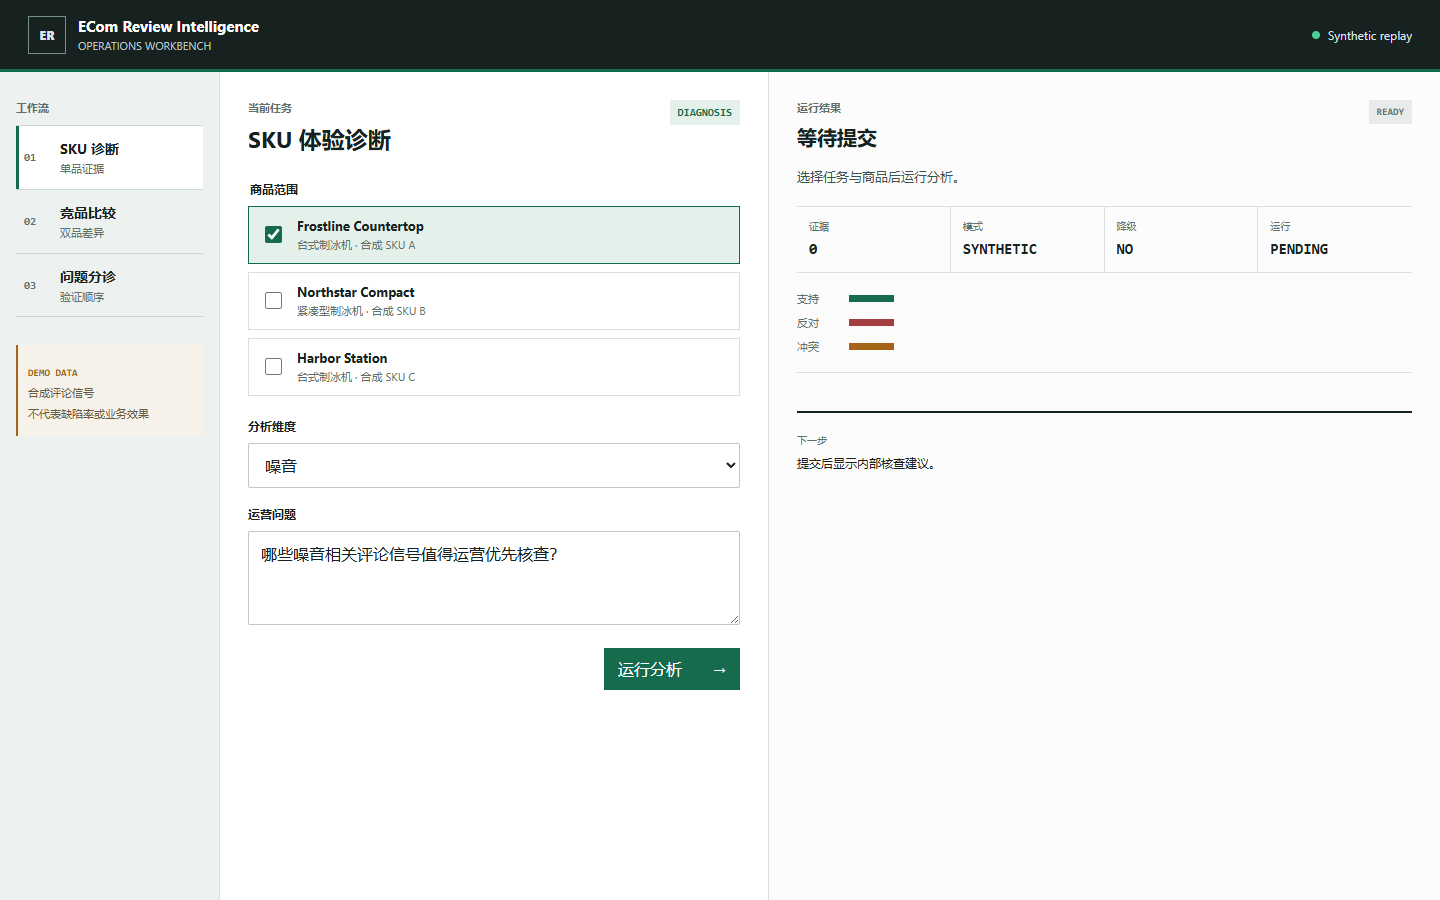
\includegraphics[width=\textwidth]{assets/p7-tour-01-initial.png}%
  }{%
    \fbox{\parbox[c][45mm][c]{0.90\textwidth}{\centering
      此处放置电脑端截图\\
      \texttt{assets/p7-tour-01-initial.png}\\
      synthetic 初始页面}}
  }
  \caption{第一次打开 synthetic 工作台：尚未提交任务。}
\end{figure}

这张图先看五个位置。\textbf{左侧工作流导航}列出单品诊断、竞品比较和问题分诊；\textbf{中间商品与问题选择}让使用者选择商品、分析维度和运营问题；页面下方的\textbf{运行按钮}负责提交这张任务单；\textbf{右侧状态}此时显示等待提交，还没有证据；右侧底部的\textbf{下一步}告诉你提交后会出现结果。\textbf{这一屏在项目中要展现什么：}使用者先从一个明确任务开始，而不是把目标交给模型自由猜。

初学者不需要一次读懂所有英文。先按“左边选任务 $→$ 中间填条件 $→$ 点击运行 $→$ 右边读结果”的方向扫一遍，再回头看细节。页面上的英文状态只是程序用来传递状态的固定标签，中文说明才是这次演示应该采取的动作。

\begin{longtable}{>{\raggedright\arraybackslash}p{0.18\textwidth}>{\raggedright\arraybackslash}p{0.31\textwidth}>{\raggedright\arraybackslash}p{0.35\textwidth}}
\toprule
位置 & 截图里看到的内容 & 先问自己的问题 \\
\midrule
\endfirsthead
\toprule
位置 & 截图里看到的内容 & 先问自己的问题 \\
\midrule
\endhead
左侧导航 & 三种任务：单品诊断、商品比较、问题分诊。 & 我现在要回答的是“看一个商品”“比较商品”，还是“决定先查哪件事”？ \\
中间表单 & 商品、分析维度、运营问题。 & 系统究竟要看谁、看哪个问题、回答什么？ \\
运行按钮 & 提交一次受控任务。 & 条件填好了吗？点击后是否会产生一次可追踪运行？ \\
右侧状态 & 等待、已验证或需要澄清。 & 结果能不能直接使用，还是要先补信息？ \\
右侧证据与下一步 & 聚合信号、证据卡和建议动作。 & 结论依据是什么？运营人员下一步要核查什么？ \\
\bottomrule
\end{longtable}

\begin{beginnerbox}
这一页的业务价值是把“我感觉这个商品可能有问题”改写成一张可以复核的任务单。任务单越明确，后面越容易知道结果回答了什么，也越容易把结果交给客服、品类或质量团队继续处理。
\end{beginnerbox}

\section{先完成一次单品诊断：看一个商品的噪声反馈}

第一次可以先保留默认的“单品诊断”（diagnosis），选择一个商品，把分析维度选为“噪音”，并将问题写成“哪些噪音相关评论信号值得运营优先核查？”。这里的商品名称只是 synthetic 页面中的演示名称，不是公开手册中的真实商品标识。

\begin{figure}[htbp]
  \centering
  \IfFileExists{assets/p7-tour-02-diagnosis.png}{%
    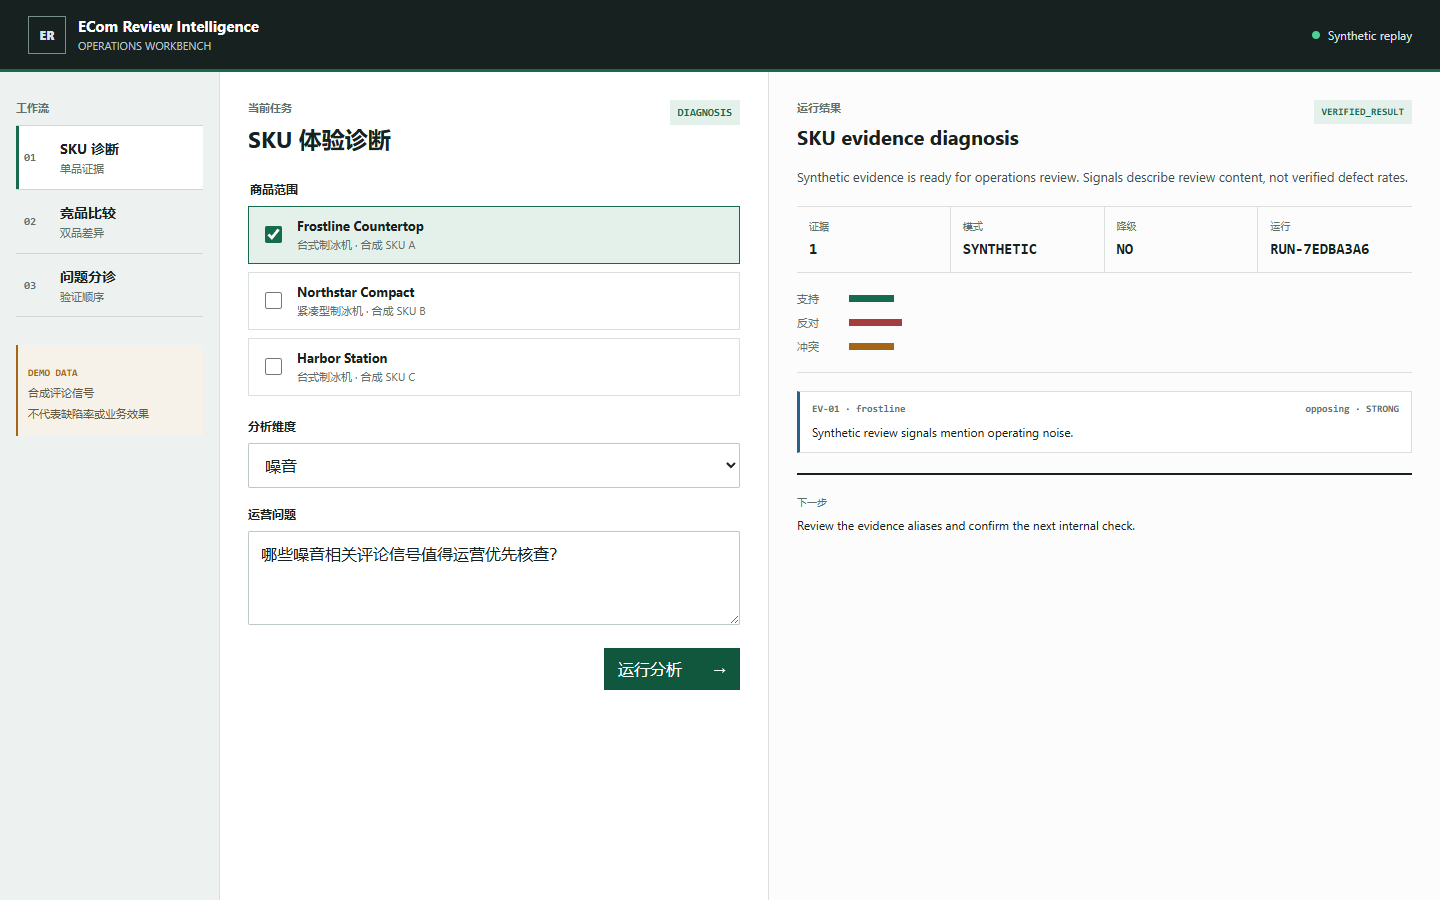
\includegraphics[width=\textwidth]{assets/p7-tour-02-diagnosis.png}%
  }{%
    \fbox{\parbox[c][45mm][c]{0.90\textwidth}{\centering
      此处放置电脑端截图\\
      \texttt{assets/p7-tour-02-diagnosis.png}\\
      单品诊断结果}}
  }
  \caption{运行单品诊断后，查看状态、证据和下一步。}
\end{figure}

这一屏中，\textbf{左侧工作流导航}高亮单品诊断；\textbf{中间区域}保留一个商品、一个分析维度和一个运营问题；\textbf{运行按钮}是任务提交的唯一入口；\textbf{右侧状态}告诉你结果是否完成检查；\textbf{右侧证据}展示匿名的聚合信号和证据卡；\textbf{右侧下一步}提示运营人员继续核查。\textbf{这一屏在项目中要展现什么：}先把“一个商品的一个问题”跑通，再理解系统如何给出可复核的证据提示。

\subsection*{结果页怎么读：先状态，后范围，再证据}

建议固定使用下面的顺序，不要先被右侧的一句英文总结带着走：

\begin{enumerate}
  \item \textbf{先看状态。}截图中的 \texttt{VERIFIED\_RESULT} 表示这次合成运行通过了本地规则检查；它表示“这份结果在当前演示边界内可继续查看”，不表示商品缺陷已经被现实世界证实。
  \item \textbf{再看范围和数量。}\texttt{SYNTHETIC} 表示数据是合成演示数据，数量表示本次允许使用的商品或证据规模；它们帮助你判断结果覆盖多大范围。
  \item \textbf{再看彩色信号条。}绿色、红色和橙色分别代表支持、反对和冲突方向。条形长短只用于比较当前演示中的相对信号，不是百分比、评分或缺陷率。
  \item \textbf{再看证据卡。}证据卡把某个信号和商品别名连起来，方便人回到本地证据账本核查；卡片中的匿名编号是本地演示 ID，不是官方 Amazon review ID。
  \item \textbf{最后看下一步。}下一步是运营动作提示，例如复核证据或确认内部检查，不是模型替人下达的采购、下架或赔付决定。
\end{enumerate}

\begin{longtable}{>{\raggedright\arraybackslash}p{0.22\textwidth}>{\raggedright\arraybackslash}p{0.34\textwidth}>{\raggedright\arraybackslash}p{0.28\textwidth}}
\toprule
右侧栏位 & 它在本项目里的功能 & 不能从它推出什么 \\
\midrule
\endfirsthead
\toprule
右侧栏位 & 它在本项目里的功能 & 不能从它推出什么 \\
\midrule
\endhead
状态 & 告诉使用者流程是否完成检查。 & 不能推出真实质量结论。 \\
范围与数量 & 说明本次运行使用的演示范围。 & 不能推出全市场样本量。 \\
信号条 & 让不同方向的聚合信号一眼可比。 & 不能当作概率、占比或 ROI。 \\
证据卡 & 给出可回查的本地证据线索。 & 不能当作原始评论全文或官方评论 ID。 \\
下一步 & 把结果交给合适的人工核查动作。 & 不能当作自动执行外部业务操作。 \\
\bottomrule
\end{longtable}

\begin{beginnerbox}
看完这张诊断图，初学者只要能回答三句话就算读懂了：\textbf{系统看的是哪个商品？它观察到的信号方向是什么？我下一步要回查哪条证据？}如果答不出来，先不要急着学习模型名称。
\end{beginnerbox}

\section{这一次运行得出了什么：把结果读成分析结论}

前面两节教的是“怎么点、按什么顺序看”。这一节回答更进一步的问题：右侧得出的这份结果，\textbf{代表了什么样的分析结论？拿到它能做什么业务动作？在项目当前阶段，它又意味着什么？}

\subsection{先分清：合成模式的数字是“演示值”，不是“计算值”}

\begin{factbox}
诊断截图中的 \texttt{EV-01}、\texttt{opposing}、\texttt{STRONG} 和三条信号条，全部来自确定性代码按固定规则生成的合成数据：单品诊断固定返回一张反对方向、STRONG 强度的证据卡。它们不来自任何真实评论的计算，因此这些数值本身没有业务含义；有学习意义的是结果的\textbf{结构}——状态、范围、方向、强度和下一步如何组合成一份可复核的结论。
\end{factbox}

这也解释了一个容易困惑的点：截图里只有一张证据卡，强度却标着 \texttt{STRONG}。在真实证据体系里，STRONG 表示“五条及以上匹配记录”；在合成模式里，它只是固定的演示标签。把“标签的定义”和“标签的来源”分开，是读懂任何模式的第一步。

\subsection{把任意一次结果读成一句结论}

无论合成、受控本地还是真实模式，都可以套用同一个结论模板：

\begin{beginnerbox}
“在〈模式标注的范围〉内，〈商品〉在〈维度〉上，系统给出〈强度〉的〈方向〉信号，下一步应〈下一步内容〉。”

套用到诊断截图即：“在合成演示范围内，Frostline 在噪音维度上给出一条 STRONG 的反对方向信号，下一步是复核证据编号并确认内部检查。”这句话就是本次运行“代表的分析结论”。注意它自带范围限定语；把限定语去掉（例如说成“Frostline 噪音有问题”），就越过了证据边界。
\end{beginnerbox}

结果页右侧各字段与结论、业务动作的对应关系如下：

\begin{longtable}{>{\raggedright\arraybackslash}p{0.18\textwidth}>{\raggedright\arraybackslash}p{0.24\textwidth}>{\raggedright\arraybackslash}p{0.24\textwidth}>{\raggedright\arraybackslash}p{0.18\textwidth}}
\toprule
字段（截图值） & 它代表的分析结论 & 拿到后可做的业务动作 & 它不能推出什么 \\
\midrule
\endfirsthead
\toprule
字段（截图值） & 它代表的分析结论 & 拿到后可做的业务动作 & 它不能推出什么 \\
\midrule
\endhead
\texttt{VERIFIED\_RESULT} & 本地检查通过、引用一致 & 继续逐卡阅读证据 & 商品质量合格 \\
模式 \texttt{SYNTHETIC} & 数字是固定演示值 & 练习读法、演示流程 & 任何真实统计 \\
证据 1 & 本次产出一卡 & 按编号回查 & 评论总数或样本量 \\
方向 \texttt{opposing} & 该卡为反对方向 & 复核客诉、补充详情页说明、列入质检关注 & 差评率 \\
强度 \texttt{STRONG} & 真实体系=五条以上匹配；合成=演示标签 & 安排核查优先级 & 问题严重度 \\
冲突信号条 & 同维度支持与反对并存（两极分化） & 人工回到原始证据下结论 & 好评差评占比 \\
下一步 & 人工核查建议 & 安排内部复核或派单 & 自动执行的动作 \\
\bottomrule
\end{longtable}

\subsection{页面英文词速查}

\begin{longtable}{>{\raggedright\arraybackslash}p{0.34\textwidth}>{\raggedright\arraybackslash}p{0.58\textwidth}}
\toprule
页面英文 & 中文含义 \\
\midrule
\endfirsthead
\toprule
页面英文 & 中文含义 \\
\midrule
\endhead
\texttt{READY} / \texttt{PENDING} & 待提交 / 等待运行 \\
\texttt{VERIFIED\_RESULT} & 已验证结果：本地校验通过，可以往下看 \\
\texttt{CLARIFICATION\_REQUIRED} & 需要澄清：商品不唯一，等人选择后继续 \\
\texttt{DEGRADED\_SAFE\_RESULT} & 安全降级：复核失败后返回的保守失败结果 \\
\texttt{SYNTHETIC} / \texttt{LOCAL} & 合成演示数据 / 受控本地真实数据 \\
\texttt{supporting} / \texttt{opposing} / \texttt{conflicting} & 支持 / 反对 / 冲突（同一维度两极分化） \\
\texttt{STRONG} / \texttt{MODERATE} / \texttt{WEAK} / \texttt{INSUFFICIENT} & 强（5 条及以上）/ 中（2--4 条）/ 弱（1 条）/ 证据不足（0 条） \\
\texttt{degraded: YES / NO} & 本次运行是否发生过安全降级 \\
\bottomrule
\end{longtable}

\subsection{三个工作流分别支撑什么业务动作}

\begin{longtable}{>{\raggedright\arraybackslash}p{0.18\textwidth}>{\raggedright\arraybackslash}p{0.40\textwidth}>{\raggedright\arraybackslash}p{0.32\textwidth}}
\toprule
工作流 & 结果支撑的业务动作 & 系统不替你做的事 \\
\midrule
\endfirsthead
\toprule
工作流 & 结果支撑的业务动作 & 系统不替你做的事 \\
\midrule
\endhead
单品诊断 & 判断是否优先复核该商品的客诉、是否在详情页补充说明、是否把该维度列入质检关注 & 不决定下架、召回或赔付 \\
竞品比较 & 为选品评审提供同一维度下的证据对比输入 & 不宣布哪个商品更好，不给采购结论 \\
问题分诊 & 决定先派给质量、客服等哪个团队，排出核查顺序 & 不自动派单，不估算业务损失 \\
\bottomrule
\end{longtable}

\begin{advicebox}
动作模板本身是真实的运营用法；但在合成阶段，证据内容是演示值，这些动作此刻只能“演练”。真实动作需要受控本地或真实模式提供可回查的证据，并经目标运营用户试用验证。
\end{advicebox}

\subsection{当前阶段，这份结果意味着什么}

\begin{factbox}
现阶段（synthetic）这份结果证明的工程事实是：任务单提交、状态标记、证据卡渲染和下一步提示的完整链路按设计工作。它是界面与流程的工程演示证据。
\end{factbox}

\begin{boundarybox}
它不证明系统对真实商品的分析正确，也不证明能节省工时或改善决策。当前项目状态为 P7 进行中：目标运营用户的结构化试用尚未完成，业务效果仍属待验证。把三种模式连起来看会更清楚：合成模式证明“页面与流程会正确地动”；受控本地模式让数字来自真实冻结数据的确定性检索与本地校验（可回查，无模型参与）；真实模型模式（命令行）再加入有预算、有边界的 LLM 参与。每前进一档，结果的业务含义才多一分；而“业务效果已验证”是最后一步，也是目前尚未完成的一步。
\end{boundarybox}

\section{再切换到商品比较：用同一个维度看差异}

理解单品诊断后，再把左侧切换到“竞品比较”（comparison），在中间勾选两个候选商品，把分析维度仍然选为“噪音”，然后点击“运行分析”。对 synthetic 演示来说，返回结果是确定的合成信号；真实模式还要经过本地证据库、工具和检查器。初学者先关注“结果有没有说明依据”，不要只看右侧的一句总结。

\begin{figure}[htbp]
  \centering
  \IfFileExists{assets/p7-tour-03-comparison.png}{%
    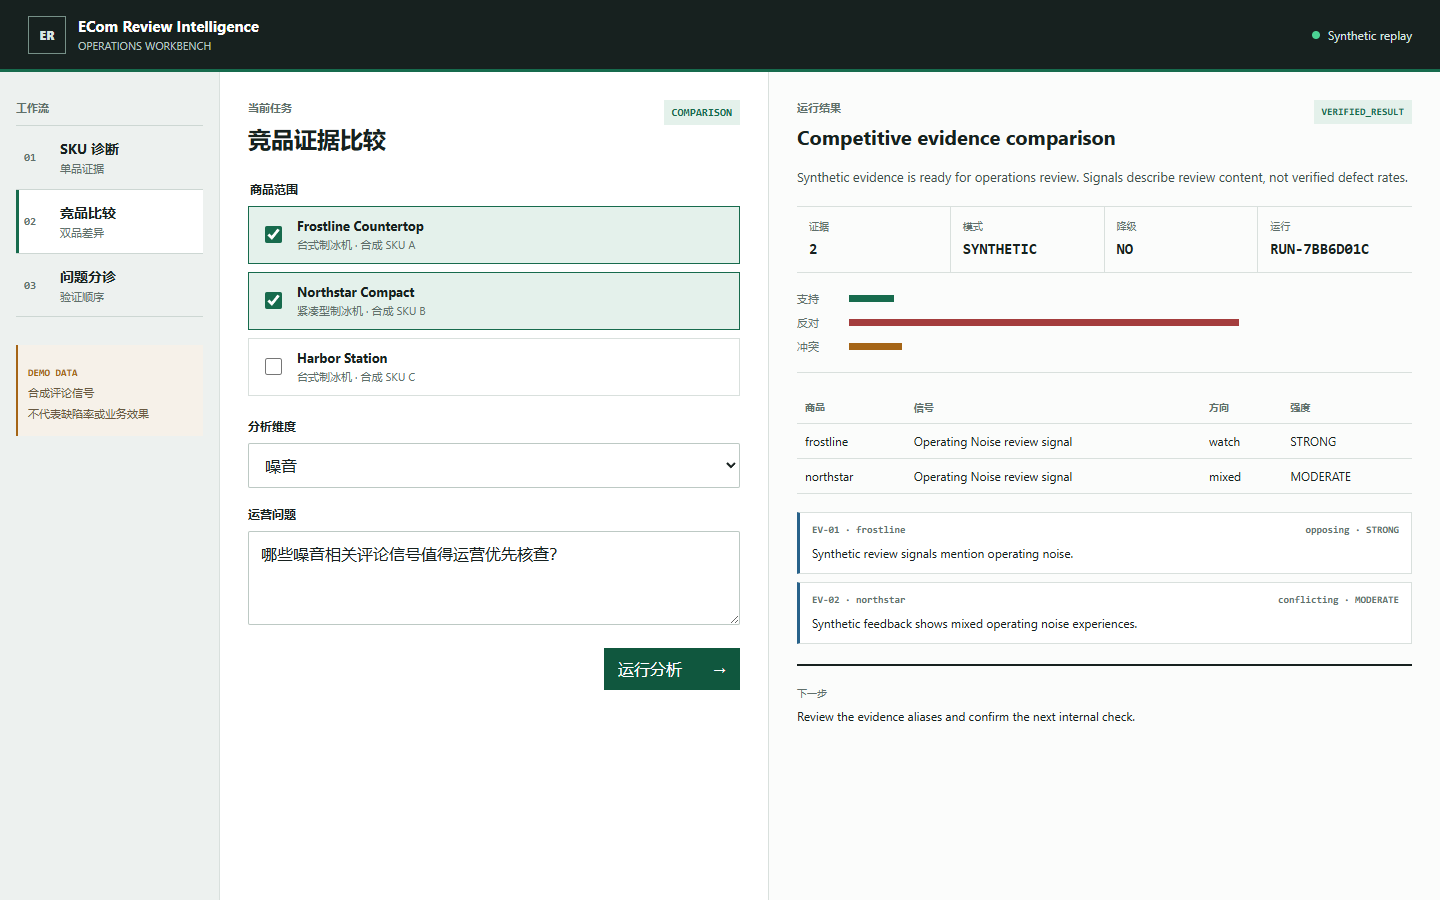
\includegraphics[width=\textwidth]{assets/p7-tour-03-comparison.png}%
  }{%
    \fbox{\parbox[c][45mm][c]{0.90\textwidth}{\centering
      此处放置电脑端截图\\
      \texttt{assets/p7-tour-03-comparison.png}\\
      比较结果、状态和证据区域}}
  }
  \caption{运行后查看状态、比较信号、证据卡和下一步。}
\end{figure}

此时，\textbf{左侧工作流导航}仍显示当前任务是竞品比较；\textbf{中间区域}保留原来的商品、维度和问题，便于回看“这份结果是在回答什么”；\textbf{运行按钮}已经触发一次受控运行，不应连续点击来制造多个不必要请求；\textbf{右侧状态}告诉你结果是否通过检查；\textbf{右侧证据}展示支持、反对或冲突的聚合信号和匿名证据卡，\textbf{下一步}给出需要运营人员继续核查的内部动作。\textbf{这一屏在项目中要展现什么：}系统输出的不只是文字，还要让人知道状态、证据数量和后续动作；它提供决策输入，不替运营人员宣布真实缺陷率。

\subsection*{比较页怎么读：先确认“同一把尺子”}

比较页最重要的不是哪一根横条更长，而是两个商品是否使用了同一个分析维度和同一类问题。截图中两个商品都放在“噪音”维度下，因此表格里的两行才有可比性。读图时依次检查：

\begin{enumerate}
  \item 中间是否真的勾选了两个商品；
  \item 下拉框中的分析维度是否相同；
  \item 右侧表格是否一行对应一个商品；
  \item 每一行能否回到自己的证据卡；
  \item 下一步是否仍然是“核查”，而不是直接宣布谁一定更好。
\end{enumerate}

这套读法的业务价值是减少“拿不同口径硬比较”的误判。例如，一个商品看噪音，另一个商品看制冰速度，即使最终文字很流畅，也不能支持采购或运营排序。比较工作流把商品范围、维度和输出行数固定下来，让运营人员知道差异来自哪里。

\begin{beginnerbox}
把比较结果先说成：“在同一个噪音维度下，两个候选商品出现了不同方向的评论信号，下一步分别回查证据。”不要说成：“A 的缺陷率比 B 高 20\%”或“A 一定应该下架”；当前截图没有这样的数据和授权。
\end{beginnerbox}

\begin{beginnerbox}
“支持、反对、冲突”是当前评论信号的方向；“证据数量”是本次允许使用的证据条数；它们都不是市场占比、缺陷率或销售损失。初次阅读时，把右侧理解成“证据提示板”即可。
\end{beginnerbox}

\section{遇到不确定时：系统先询问，而不是替你猜}

如果使用者没有指定唯一商品，只输入了一个可能对应多个商品的宽泛说法，系统会进入澄清状态。澄清不是报错，而是把必须由人决定的选择显式展示出来。

\begin{figure}[htbp]
  \centering
  \IfFileExists{assets/p7-tour-04-clarification.png}{%
    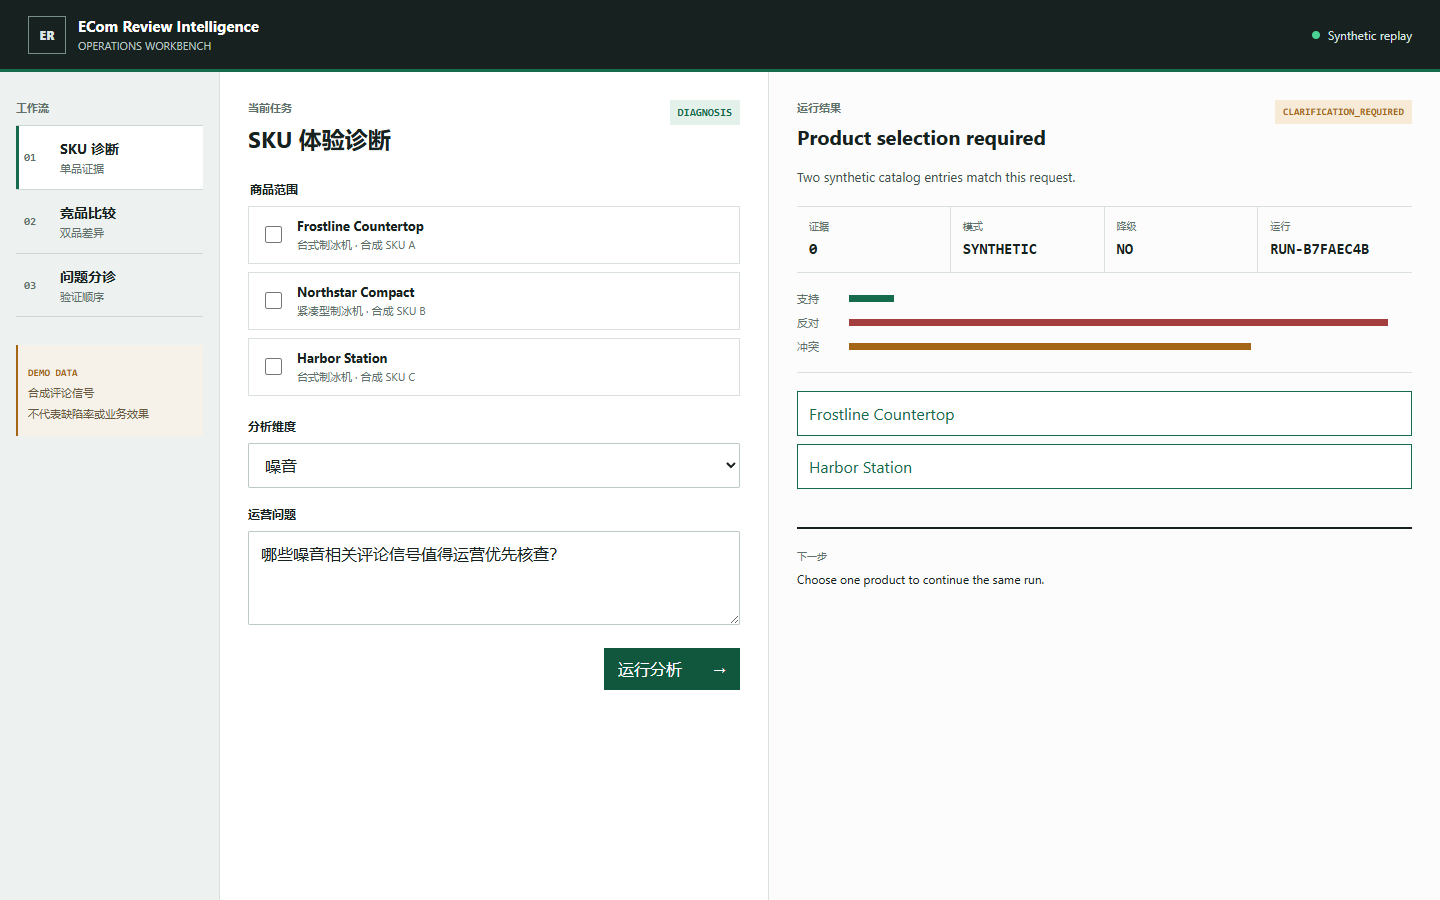
\includegraphics[width=\textwidth]{assets/p7-tour-04-clarification.png}%
  }{%
    \fbox{\parbox[c][45mm][c]{0.90\textwidth}{\centering
      此处放置电脑端截图\\
      \texttt{assets/p7-tour-04-clarification.png}\\
      需要选择候选商品的澄清页面}}
  }
  \caption{商品有多个候选时，进入澄清状态并选择授权候选。}
\end{figure}

这张图中，\textbf{左侧工作流导航}仍保留原任务类型；\textbf{中间商品与问题区域}显示原来填写的任务条件，并等待你从候选商品中作选择；\textbf{运行按钮}不会通过重复提交绕过选择；\textbf{右侧状态}明确显示需要澄清；\textbf{右侧证据与下一步}暂不假装有最终结论，而是告诉你先完成候选选择。\textbf{这一屏在项目中要展现什么：}当输入不够明确时，系统把决策交还给使用者，并保存这次任务以便继续。

澄清完成后，使用者点击一个已授权候选，系统恢复同一任务继续运行。这就是 checkpoint（暂停时保存的任务状态）最直观的含义：它像一张暂存的工作单，不需要从头猜一遍，也不允许选择候选列表之外的商品。

\subsection*{澄清页怎么读：这是安全功能，不是系统坏了}

澄清页右侧没有最终证据卡，是因为“到底分析哪个商品”这个前提还没有确定。它把模型不能安全替人决定的部分显式交还给使用者。对运营来说，这能避免把甲商品的评论误归到乙商品上；对工程来说，这能把一次运行停在明确状态，等人选择后再从原位置继续。

看到 \texttt{CLARIFICATION\_REQUIRED} 时，按三步处理：

\begin{enumerate}
  \item 看候选列表，确认每个候选的名称和上下文；
  \item 选择自己有权限确认的商品，不要凭相似名称猜测；
  \item 回到同一个运行，继续看状态、证据和下一步。
\end{enumerate}

这张图体现的价值是“宁可多问一次，也不把错误对象的证据交给业务”。它也是后面学习 checkpoint、恢复、审计和人工接管的最直观入口。

\section{从简单到完整：你正在逐渐学会哪些功能}

不要把工作台理解成一次性学会的“大模型聊天框”。可以按下面的能力梯度学习：

\begin{longtable}{>{\raggedright\arraybackslash}p{0.16\textwidth}>{\raggedright\arraybackslash}p{0.33\textwidth}>{\raggedright\arraybackslash}p{0.33\textwidth}}
\toprule
学习顺序 & 先学会什么 & 学会后的实际作用 \\
\midrule
\endfirsthead
\toprule
学习顺序 & 先学会什么 & 学会后的实际作用 \\
\midrule
\endhead
第 1 步 & 填写商品、维度和运营问题。 & 把模糊需求写成可执行任务。 \\
第 2 步 & 看状态、数量和证据卡。 & 判断结果是否有依据、是否需要人工复核。 \\
第 3 步 & 用同一维度比较多个商品。 & 给品类或运营团队提供可回查的差异线索。 \\
第 4 步 & 处理澄清和恢复。 & 遇到歧义时不猜错对象，并能继续原任务。 \\
第 5 步 & 理解工具、Verifier 和 Trace。 & 知道结果怎样被检索、检查和记录。 \\
第 6 步 & 连接真实 API 或真实用户试用。 & 在满足额外门槛后，评估延迟、成本和真实业务可用性。 \\
\bottomrule
\end{longtable}

前四步是“会用”；第五步是“能解释为什么相对可靠”；第六步才是“有资格讨论真实效果”。当前手册已经把前五步放进项目流程，但截图仍是 synthetic 演示，真实 API 和目标运营用户试用不应被截图替代。

\section{为什么页面有三种工作流}

三种工作流不是三个互相独立的 Agent，而是运营人员常见的三种问题形状。把它们分开，是为了让商品数量、输出形式和下一步动作都清楚。

\begin{longtable}{>{\raggedright\arraybackslash}p{0.22\textwidth}>{\raggedright\arraybackslash}p{0.32\textwidth}>{\raggedright\arraybackslash}p{0.32\textwidth}}
\toprule
页面任务 & 它回答什么 & 为什么不能混在一起 \\
\midrule
\endfirsthead
\toprule
页面任务 & 它回答什么 & 为什么不能混在一起 \\
\midrule
\endhead
单品体验诊断（diagnosis） & 一个商品在某个体验维度上有哪些支持、反对或冲突信号？ & 重点是看清一个商品的问题，不需要强行找出另一个商品。 \\
竞品证据比较（comparison） & 两个或多个商品在同一个维度上的证据有什么差异？ & 必须使用相同维度，否则比较的不是同一件事。 \\
问题分诊（triage） & 哪个运营问题值得先交给相应团队核查？ & 输出的是调查顺序，不等于缺陷严重度或财务损失排序。 \\
\bottomrule
\end{longtable}

如果把三种任务混成一个万能聊天框，模型可能既回答“这个商品怎么样”，又直接说“应该选哪个”，还把“先核查什么”说成“最严重的问题”。分开后，使用者能在运行前确认任务类型，程序也能为每种任务检查正确的商品数量和输出字段。

\section{把页面重新接回 P0--P7}

刚才的任务看起来只是勾选商品、选择维度和点击按钮，但页面背后依赖前面阶段已经做好的边界。可以按下面的顺序理解：

\begin{longtable}{>{\raggedright\arraybackslash}p{0.16\textwidth}>{\raggedright\arraybackslash}p{0.29\textwidth}>{\raggedright\arraybackslash}p{0.39\textwidth}}
\toprule
阶段 & 在刚才的任务中负责什么 & 初学者先这样理解 \\
\midrule
\endfirsthead
\toprule
阶段 & 在刚才的任务中负责什么 & 初学者先这样理解 \\
\midrule
\endhead
P0/P1 & 保证输入 & 先确认数据能用，再保证每次分析使用的是同一版输入。 \\
P2/P3 & 定义范围和维度 & 决定本项目看哪个类目，以及“噪音”这类问题怎样划分和标记。 \\
P4 & 提供证据 & 把允许使用的评论信号放进一个可以反复查询的本地证据账本。 \\
P5 & 比较检索 & 检查怎样更稳定地找到相关证据，比较方法是否真的引用了正确商品。 \\
P6 & 组织 Agent & 让模型按任务单规划，调用有限工具，并在出结果前接受复核。 \\
P7 & 提供工作台 & 把前面的能力放到电脑网页上，让运营人员可以填写任务、查看状态和继续澄清。 \\
\bottomrule
\end{longtable}

这也解释了为什么不能一开始就只写一个聊天框：如果 P0/P1 没有可靠输入，P2/P3 没有统一维度，P4 没有证据，P5 没有比较基线，P6 的 Agent 就算写出流畅答案，也不知道答案能不能被复核。P7 只是把已经有边界的能力呈现出来，并没有把演示页面变成业务效果证明。

\section{这一章学到什么，后面怎样读}

第一次使用时，你只需要掌握这条操作线：\textbf{选任务} $\rightarrow$ \textbf{选商品和维度} $\rightarrow$ \textbf{写运营问题} $\rightarrow$ \textbf{运行} $\rightarrow$ \textbf{看状态和证据} $\rightarrow$ \textbf{按下一步继续核查}。遇到多个商品命中时，先澄清再继续。

后面阅读 P0--P7 时，每一阶段都可以回到这个完整任务：这一阶段为页面中的哪一部分提供了保证？它解决了什么风险？如果拿掉它，右侧结果会失去什么可信度？这样学习路线就从“先学抽象 Agent”变成“先看一个业务任务，再逐步理解它为什么能够安全运行”。

\begin{interviewbox}
面试时可以这样介绍：“我先用一个竞品噪音反馈比较任务说明工作台的使用方式：运营选择两个商品和同一体验维度，运行后查看状态、聚合信号和可回查证据；输入有歧义时，系统先澄清并恢复原任务。这个页面是 P0--P6 的能力在 P7 的呈现，synthetic 截图只证明演示流程，不代表真人业务效果已经验证。”
\end{interviewbox}

\chapter{系统路线图：从来源可行到运营工作台}

\section{先看一条完整的因果链}

这个项目不是先做一个 Agent，再回头寻找它可以使用的数据。开发顺序是一条不可跳步的依赖链：

\begin{center}
来源可行性 $\rightarrow$ 冻结快照 $\rightarrow$ 限定类目 $\rightarrow$ 证据合同 $\rightarrow$
本地证据引擎 $\rightarrow$ 检索基线 $\rightarrow$ 受约束 Agent $\rightarrow$ 运营工作台
\end{center}

每一步只解决一个新的不确定性。后一步必须继承前一步的输入身份和边界，不能因为界面更完整或模型能生成流畅文本，就改写上游数据事实。

\begin{beginnerbox}
可以把这条链理解成建造一条可审计的生产线：P0 确认原料来源和工作条件；P1 封存本次使用的原料；P2 决定只做哪个业务范围；P3 规定什么可以叫证据；P4--P5 负责稳定取证和比较方法；P6 让模型在规则内协作；P7 才把能力交给运营人员试用。
\end{beginnerbox}

\section{八个阶段的输入、能力、闸门与交接}

\small
\begin{longtable}{@{}>{\raggedright\arraybackslash}p{0.06\textwidth}>{\raggedright\arraybackslash}p{0.18\textwidth}>{\raggedright\arraybackslash}p{0.20\textwidth}>{\raggedright\arraybackslash}p{0.18\textwidth}>{\raggedright\arraybackslash}p{0.18\textwidth}@{}}
\toprule
阶段 & 输入 & 新增能力 & Gate & 交给下一阶段 \\
\midrule
\endfirsthead
\toprule
阶段 & 输入 & 新增能力 & Gate & 交给下一阶段 \\
\midrule
\endhead
P0 & 官方来源说明、字段需求、本地环境 & 有界来源探测与资源预检 & 来源、环境、容量及公开边界可行 & 经核实的来源角色与限制 \\
P1 & P0 认可的评论与元数据来源 & 可恢复下载、完整性登记和冻结快照 & 两个角色完整且 manifest 原子发布 & 按角色读取的冻结输入 \\
P2 & P1 manifest & 流式质量审计与类目决策 & 精确关联、覆盖和选择理由可审查 & Ice Makers 范围及审计身份 \\
P3 & P2 范围与真实字段 & 冻结证据口径和标签来源 & 八个 aspect、极性、强度与引用规则冻结 & 带 lineage 的证据合同 \\
P4 & P1--P3 冻结身份 & SQLite/FTS5 本地证据引擎 & 精确关联、稳定引用、原子建库 & 可确定性查询的证据服务 \\
P5 & P4 引擎与冻结案例 & 同基准检索比较 & 引用、关联、无答案和延迟门 & 是否增加检索复杂度的证据 \\
P6 & P3--P5 合同、工具与基线 & 受约束单 Agent 和 Verifier & 离线、真实模型及完成审计的有界工程门 & 结构化、安全的任务结果 \\
P7 & P6 图、工具、验证器和公开 DTO & 本地运营工作台 & 工程验证完成；真人结构化试用仍开放 & 用户验证记录与下一轮产品决策 \\
\bottomrule
\end{longtable}
\normalsize

\section{状态不是业务成功证明}

\begin{factbox}
当前仓库中，P0--P6 的阶段状态为 PASSED。这个状态只表示对应冻结输入和规定 Gate 已满足，不表示销量、利润、缺陷率、用户采纳或生产 SLA 已获证明。

P7 仍为 \statusprogress，因为目标运营用户的结构化试用尚未完成。
\end{factbox}

\begin{boundarybox}
路线图中的箭头表示工程依赖，不表示因果业务效果。尤其是 P7 尚缺目标运营用户的结构化试用，因此当前不能声称工作台节省了真实工时或改善了决策质量。
\end{boundarybox}

\section{怎样使用后面的阶段章节}

P0--P7 采用同一套阅读模板：先看“承上启下”和业务问题，再沿“开发过程”理解为什么这样实现；随后学习技术知识、复盘问题与修复、核对验收边界，最后练习如何进入下一阶段和如何在面试中准确表达。初学者应按顺序阅读，因为 P6 的 Agent 权限来自 P3--P5，而不是模型自身。

\chapter{P0：先确认数据能不能放心用}

\section{承上启下}

在项目起点，我们还没有一批可以放心使用的数据，也没有资格讨论检索或 Agent。P0 的任务是回答一个更基础的业务问题：\textbf{投入下载和开发之前，来源、字段、本地资源与公开边界是否足以支持一个本地证据原型？}

\section{输入、边界与价值}

\textbf{输入}包括官方数据说明、评论与元数据的最低字段需求、预期文件规模、本地 Python 与磁盘条件，以及公开作品集的目标。用运营语言说，就是先确认“数据从哪里来、里面有没有后面要用的内容、我的电脑能不能处理、哪些内容不能公开”。

\textbf{边界}是只做有界预检，不下载完整数据，不检查评论内容质量，也不证明数据可以公开再分发。P0 带来的业务价值是提前暴露资源和合规风险；技术价值是把环境与来源假设变成可重复检查的证据。

\begin{boundarybox}
“公开可访问”只说明当前能够从公开端点取得响应，不等于数据附带再分发许可。任何评论衍生文本的公开展示仍需单独的数据使用审查；原始数据继续留在本地且不进入 Git。
\end{boundarybox}

\section{开发过程}

\subsection{1. 把模糊可行性拆成四个问题}

P0 分别检查来源可达性、字段可用性、运行环境和容量，并把官方事实、现场观察、设计决定、开放问题和阻塞项分开记录。这样，后来即使来源或环境变化，也能知道需要重查哪一项。这里的重点不是写复杂脚本，而是把“我觉得应该可以”变成几项能重新检查的事实。

\subsection{2. 先用很小的请求探测来源}

项目对评论和元数据来源各请求一个很小的字节范围。通俗地说，这像先确认仓库门能打开、标签与预期一致，而不是立即把整批货搬回家。观察到的部分内容响应与 gzip 类型，只支持“当时的端点可达且对象形态符合预期”这一有限结论。

\subsection{3. 检查本地环境和容量}

预检确认支持的 Python、操作系统和可用空间能够覆盖预计下载与后续处理需求。容量估算必须为压缩输入、临时文件和派生产物留出空间，不能只比较压缩包大小。

\subsection{4. 先写公开边界}

公开版本只允许代码、合成夹具、聚合结果和经审查的文档。原始评论、真实标识、密钥、大型索引和本地路径从一开始就被排除，而不是发布前临时清理。

\section{本阶段学到的知识}

\textbf{有界探测}用最小网络和存储成本验证关键假设；\textbf{容量预检}避免流程中途失败；\textbf{事实分层}防止把观察、决策和推断混在一起；\textbf{数据可用性与许可分离}则是公开项目的治理基础。换成初学者的话：先小范围检查，再决定是否值得投入时间和空间。

\begin{beginnerbox}
项目例子：两个来源都对一字节范围请求返回有效响应，只能说明 P0 当时观察到“可达”。它不能证明完整文件已经下载，不能证明内容正确，也不能代替许可证判断。
\end{beginnerbox}

\section{问题、修复与验证}

最危险的误解是“能下载，所以能公开”。修复不是猜测许可，而是缩小公开面，并在报告中保留“公开展示需另行审查”的开放问题。验证则重新执行有界来源探测、Python 与容量检查，确认没有当前阻塞项。

\textbf{小练习：}把“端点返回部分内容”改写成三种句子：可声称、不可声称、仍待核实。合格答案应把可达性、完整下载和再分发权分开。

\section{阶段产出与验收边界}

P0 的权威产出是 \filelink{docs/reports/phase-0-preflight.md}。其 Gate 证明的是：在记录时点，官方来源有界可达，环境和容量满足当前计划，公开边界已有设计。它不证明完整数据质量、再分发权、业务需求或任何商业效果。P0 在这一边界内为 \statuspassed。

\section{怎样进入下一阶段}

P1 只能使用 P0 核实过的两个来源角色，开始可恢复取得和完整性登记。若来源身份、所需字段或容量条件变化，应先重跑 P0，而不是直接把新文件塞进原始目录。

\section{面试怎么讲}

\begin{interviewbox}
“我没有直接下载数据或搭 Agent，而是先用有界请求验证两个官方来源，并检查 Python、容量和公开边界。这个阶段只证明项目在当前条件下可开展；公开可访问不等于有再分发许可，所以原始数据保持本地，评论衍生文本仍需单独审查。”
\end{interviewbox}

\textbf{掌握标准：}能够解释 P0 的四项检查，并明确说出至少三项它没有证明的结论。

\chapter{P1：保证后面一直使用同一版数据}

\section{承上启下}

P0 只证明来源和本地条件可行，尚未形成可复现输入。P1 的业务问题是：\textbf{怎样保证后续每个阶段使用的是同一对评论与元数据文件，而不是某次中断、替换或误发现的文件？}

\begin{beginnerbox}
继续沿用 P0 的运营例子：如果今天的“漏水”结论来自文件 A，下周却不小心读了同名的文件 B，就无法判断变化来自商品还是来自数据。P1 要做的就是给本次输入做一份清单和版本记录；以后要换数据，必须明确换一版。
\end{beginnerbox}

\section{输入、边界与价值}

输入是 P0 核实过的评论和元数据来源角色。P1 不解释评论内容、不选择品类，也不声称拥有服务端官方 checksum。业务价值是让不同时间的分析仍能回答“用了哪批输入”；技术价值是把下载恢复、并发安全、完整性与发布原子性组成一条证明链。这里的“冻结”不是把文件锁死，而是给当前版本盖章，避免下游偷偷换文件。

\section{开发过程}

\subsection{1. 继续下载前先确认还是同一个文件}

断点续传不是简单地从旧文件末尾继续写。流程先比较远端对象身份，例如对象标签或最后修改时间；只有身份仍与已记录对象一致，Range 恢复才有意义。远端身份变化时必须停止，避免把两个版本拼成一个文件。初学者可以先把它理解为：搬货搬到一半回来，先确认仓库里的货没有换批次。

\subsection{2. 保证同一时间只有一个下载者}

同一目标在同一时间只允许一个写入者。独占锁拒绝第二个下载进程；遗留锁不能静默删除，而要经过显式恢复。这里的锁保护的是并发行为，不是数据正确性的替代品。它解决的是“两个人同时往同一个箱子里装东西”的问题。

\subsection{3. 检查文件完整，再留下文件指纹}

下载或人工取得后，先完整读取 gzip 流，检查压缩结构没有截断；再计算本地内容哈希，作为以后重新核对同一字节内容的文件指纹。人工直接下载的记录只支持本地大小、gzip 与哈希均通过，不伪装成已捕获浏览器 HTTP 回执或平台官方校验和。

\subsection{4. 给两类文件做一份输入清单（manifest）}

评论与元数据两个角色全部通过后，才生成组合快照 manifest。manifest 可以先理解为“输入清单”：同时记录角色、来源身份、本地完整性和快照身份。下游读取“reviews”“metadata”等角色映射，而不是扫描原始目录猜哪个文件最新。

\subsection{5. 只有整批检查通过才发布}

manifest 先写临时文件，内容完整并通过检查后再替换正式文件。如果任一输入失败，旧的有效 manifest 不应被半成品覆盖。通俗地说，公开的是一张完整封条，而不是边写边让下游读取的草稿。这类“要么整批成功、要么不换旧版本”的动作，工程上叫原子发布。

\section{本阶段学到的知识}

本阶段把\textbf{可恢复传输、远端对象身份、跨进程锁、gzip 流校验、本地哈希、manifest 和原子发布}串成一个系统。初学者先掌握一句话：先确认没有换批次，再确认文件没损坏，最后把通过检查的整批输入登记下来。单独拥有哈希并不能证明来源官方背书；单独拥有锁也不能证明文件完整。只有这些机制按顺序组合，才能给下游稳定输入。

\begin{beginnerbox}
项目例子：假设原始目录里多出一个名字相似的压缩包。P2 不能因为它“更新”就读取它，而必须从冻结 manifest 的角色字段解析输入。这样文件命名或目录噪声不会悄悄改变数据快照。
\end{beginnerbox}

\section{问题、修复与验证}

问题一是中断下载可能留下可读但不完整的 gzip；修复是完整流校验。问题二是并发写入或遗留锁可能污染目标；修复是默认拒绝第二写入者和显式恢复。问题三是人工下载缺少服务端 checksum；修复是诚实限定为本地观察。最后通过失败场景验证：角色缺失、身份变化或完整性失败时，不发布新快照。

\textbf{小练习：}说明“本地 SHA-256 相同”和“平台提供官方 checksum”为什么不是同一断言。前者证明两次本地字节计算一致，后者还要求可核实的服务端声明。

\section{阶段产出与验收边界}

主要产出为 \filelink{artifacts/manifests/phase-1-download.json} 与 \filelink{docs/reports/phase-1-download.md}。P1 Gate 要求两个最终 gzip 角色完整、本地哈希已登记、组合快照原子发布，并发写入受到约束。它不证明浏览器传输过程、服务端官方 checksum、内容语义质量或公开再分发权。P1 在该边界内为 \statuspassed。

\section{怎样进入下一阶段}

P2 必须按 manifest 中的角色读取输入，并在解析前重算本地哈希。任何未登记文件都不能自动加入审计；若要更换数据，必须重新形成 P1 快照，而不是在 P2 临时换源。

\section{面试怎么讲}

\begin{interviewbox}
“我把下载、登记和发布分开：恢复前检查远端身份，写入用独占锁，完成后验证整个 gzip 并计算本地哈希，最后原子发布同时包含评论和元数据角色的冻结 manifest。下游只按 manifest 角色读取，不扫描原始目录。我不会把本地哈希说成官方 checksum。”
\end{interviewbox}

\textbf{掌握标准：}能够画出“身份检查 $\rightarrow$ 恢复 $\rightarrow$ 锁 $\rightarrow$ gzip $\rightarrow$ 哈希 $\rightarrow$ manifest $\rightarrow$ 原子替换”的失败关闭路径。

\chapter{P2：从全量数据找到适合解决的业务范围}

\section{承上启下}

P1 已经确认了一批可以重复使用的数据。现在的新问题不是“还有多少文件”，而是“先服务哪一类商品，运营问题才最清楚”。P2 因此要从全量数据中选出一个可以学习、可以检索、可以做运营演示的范围。

\section{业务问题、输入与边界}

业务问题是：哪些候选类目同时有足够商品、足够评论和足够的字段覆盖，能够支持单品诊断、竞品比较和问题分流？输入只能来自 P1 登记过的评论和商品文件。

这里的价值要先说清楚。\textbf{业务价值}是避免一开始就凭兴趣选类目，减少后续返工；\textbf{技术价值}是学会在大文件上做可重复的质量检查。P2 不证明任何商品真的更好，也不估计销量、缺陷率或商业收益。

\section{开发过程}

\subsection{1. 先确认没有偷偷换数据}

脚本先检查 P1 的数据指纹和登记清单。可以把它理解成进仓前核对“这是不是之前登记的那批货”。如果文件内容已经变化，流程停止，而不是看到同名文件就继续。

\subsection{2. 一行一行检查大文件}

评论文件很大，不能为了统计就把全部内容一次塞进内存。程序逐行读取，记录格式是否正确、字段是否存在、评分和时间是否合理、评论能否找到对应商品。这种边读边统计的方法叫\textbf{流式审计}，先理解为“大文件的流水点数”。

\subsection{3. 只用明确的商品键关联}

评论和商品资料通过冻结的父商品键连接，不通过相似标题猜测。结果显示商品资料 94,327 行、评论 2,128,605 行，其中 2,100,939 条评论被精确关联，27,666 条未关联。这里的“关联”只说明源字段一致，不是对现实商品身份的独立认证。

\subsection{4. 让算法给出建议，再由业务目标做选择}

先设置最少商品数、最少评论数和覆盖门槛，再按固定权重给候选范围排序。算法建议 Water Filters；Ice Makers 也满足门槛，并且更容易围绕制冰质量、噪声、可靠性、清洁、速度、安装、漏水和便携性组织运营问题，所以项目选择 Ice Makers。

这个选择记录为一个\textbf{业务覆盖决策}（override）：不是把算法改到“刚好选中 Ice Makers”，而是在合格候选中公开说明为什么选择它。最终范围包含 3,278 个商品和 136,604 条精确关联评论，文本覆盖为 0.998675。

\section{本阶段学到的知识}

\begin{itemize}
  \item \textbf{流式审计：}像流水线点数，适合大文件，且不制造完整解压副本。
  \item \textbf{精确关联：}像用订单号找订单，不用商品标题相似度猜测。
  \item \textbf{候选评分：}把“数据适不适合做项目”变成可以比较的规则。
  \item \textbf{业务覆盖决策：}算法建议和产品选择可以不同，但理由必须留下。
\end{itemize}

\begin{beginnerbox}
项目例子：Water Filters 分数更高，是数据规则给出的建议；Ice Makers 被选择，是带理由的产品范围决定。两者都可以是真实记录。真正的问题是事后偷偷改权重，却不告诉读者。
\end{beginnerbox}

\textbf{小练习：}如果某个类目故事很好讲，但评论覆盖没有达到最低门槛，能不能直接选？不能。业务判断可以在合格候选中做，不能绕过数据检查。

\section{问题、修复与验证}

最容易出现的错误，是把“最高分”误解成“唯一正确答案”。修复是同时保留算法推荐、合格门槛、最终选择和选择理由。验证包括重新核对数据指纹、格式和关联统计、覆盖门槛、候选排序及范围登记。

\section{阶段产出与验收边界}

产出包括\filelink{artifacts/audits/phase-2-audit.json}、\filelink{artifacts/manifests/phase-2-scope.json}和\filelink{docs/reports/phase-2-audit.md}。P2 在其范围内为\statuspassed：说明选定的 Ice Makers 范围来自合格数据且过程可追踪；不说明它的商业价值已经被证明，也不说明评论代表全部消费者。

\section{怎样进入下一阶段}

P3 要在这批 Ice Makers 数据上规定“什么可以算作证据”：例如噪声、漏水怎样分类，支持和反对怎样区分，结果怎样引用。P3 必须继续使用本阶段的范围登记，不能看到后面的结果后重新选类。

\section{面试怎么讲}

\begin{interviewbox}
“我先在固定输入上逐行审计和精确关联，再按门槛和固定权重比较候选。算法推荐 Water Filters，但我选择了同样合格、且更适合三个运营工作流的 Ice Makers，并把这个业务决策和理由单独记录，没有反向调整参数迎合结论。”
\end{interviewbox}

\textbf{掌握标准：}能分开说清楚“数据观察”“算法建议”和“业务选择”，并说明它们各自的证据来源。

\chapter{P3：先约定什么算证据}

\section{承上启下}

P2 选出了 Ice Makers，但“评论里出现一个词”还不能直接变成运营结论。P3 要先回答：不同程序和不同时间分析评论时，是否遵守同一套说法？这一步像先制定一本共同的评分规则，再开发查询工具。

\section{业务问题、输入与边界}

输入是 P1 的数据记录、P2 的范围记录和审计结果。业务价值是让不同商品的 VOC 结果可以比较、可以回查；技术价值是把字段、分类和引用方式写成下游程序能够检查的约定。

P3 不训练模型，不做人类金标准标注，也不把评论信号直接说成现实缺陷或因果影响。它规定的是“我们怎样描述当前数据中的信号”。

\section{开发过程}

\subsection{1. 先规定每条评论看哪些字段}

规则明确商品键、评论商品键、文本、评分、时间、购买标记和帮助票如何对应，并继续带上 P1--P2 的来源记录。这个从输入到结果的来路记录叫\textbf{lineage}，可以先理解为“结果的家谱”。

\subsection{2. 把运营问题分成八个体验维度}

项目使用八个 aspect（体验维度）：\texttt{ice\_quality}、\texttt{noise}、\texttt{reliability}、\texttt{cleaning\_maintenance}、\texttt{capacity\_speed}、\texttt{ease\_setup}、\texttt{leakage} 和 \texttt{size\_portability}。例如“机器很吵”进入 noise，“清洗麻烦”进入 cleaning\_maintenance。维度名称是给程序用的固定标签；模型不能临时创造第九个维度并当成既定事实。

\subsection{3. 区分支持、反对和冲突}

词表把当前匹配到的内容记录为支持、反对或冲突信号。这是对本批评论的描述，不是通用情感评分，更不是“已经确认产品有缺陷”。

\subsection{4. 用证据条数表达强弱}

0 条为 \texttt{INSUFFICIENT}，1 条为 \texttt{WEAK}，2--4 条为 \texttt{MODERATE}，5 条及以上为 \texttt{STRONG}。这些等级只表示匹配记录数量，不会自动消除重复表达、样本偏差或评论真实性问题。

\subsection{5. 给每条本地证据一个可回查的编号}

本地 evidence ID 由数据版本、来源角色和源记录位置确定性生成。同一批输入重新计算时，仍能找到同一位置。这是项目内部的定位编号，不是 Amazon 官方评论 ID，不能公开冒充平台标识。

\subsection{6. 记录标签是怎么来的}

\textbf{silver} 是规则或测试产生的确定性期望，适合回归检查但未经人工确认；\textbf{reviewed} 需要实际人工审核记录；当前不能声称 \textbf{gold}，因为项目没有独立、充分且一致的人类金标准。

\section{本阶段学到的知识}

\textbf{数据合同}就是“程序共同遵守的表格和语义规则”；\textbf{contract identity} 是这套规则的版本号；\textbf{lineage} 是结果的来路；稳定本地 ID 是可回查的门牌号；\textbf{label provenance} 是标签来源说明。它们共同限制系统能说什么、不能说什么。

\begin{beginnerbox}
项目例子：某商品在 noise 维度下有多条反对信号，可以说“这批冻结评论中存在较强噪声相关信号”。不能直接说“商品已被证明存在噪声缺陷”，因为两句话的证据范围不同。
\end{beginnerbox}

\textbf{小练习：}一条规则结果连续通过测试，但从未有人审核，它是什么标签？答案仍是 silver；测试稳定不等于人工真值。

\section{问题、修复与验证}

主要问题是把词频、情绪、问题信号、缺陷和商业影响混成一个词。修复是分开记录体验维度、极性、强度和标签来源，并在输出中保留限定语。另一个问题是下游各自复制规则并悄悄修改，修复方式是保存合同身份并检查 lineage。验证覆盖八个维度、强度边界、极性词表、字段映射、标签政策和本地引用可重算性。

\section{阶段产出与验收边界}

权威产出是\filelink{artifacts/contracts/phase-3-evidence-policy.json}和\filelink{docs/decisions/phase-3-evidence-policy.md}。P3 在其范围内为\statuspassed：八个维度、极性、强度、引用和标签来源规则已经固定；不证明规则达到人工标注质量，也不证明评论信号对应现实缺陷。

\section{怎样进入下一阶段}

P4 将把这些规则放进本地证据工具，让程序快速找到商品和评论，并能回查引用。P4 可以改变实现方式，但不能重新解释本阶段的维度、极性、强度或标签来源。

\section{面试怎么讲}

\begin{interviewbox}
“在做检索和 Agent 前，我先冻结证据合同：八个体验维度、词法极性、按记录数定义的强度、本地稳定引用和标签来源都由代码校验。下游必须携带同一 lineage。规则结果只叫 silver，本地 evidence ID 也不是平台官方评论 ID。”
\end{interviewbox}

\textbf{掌握标准：}能用一个评论例子解释数据合同怎样约束后面的检索、Agent 和网页结果，并区分“可回查”“人工复核”和“现实真值”。

\chapter{P4：把评论变成可以反复查询的证据工具}

\section{承上启下}

P3 已经说清楚什么算证据，但每次都从大量原始文件翻找，运营人员和后续 Agent 都会很慢，也容易引用错商品。P4 要做一个本地“证据账本”：输入同样的问题，尽量得到同样的可回查证据。

\section{业务问题、输入与边界}

业务问题是：怎样快速找到某个商品、某个体验维度的支持或反对信号？输入是 P1 冻结数据、P2 选定范围、P3 证据合同和本地原始文件。输出是受控的本地证据服务，不是自动生成商业结论。

业务价值是减少重复翻评论的时间，并让运营人员知道结论来自哪里；技术价值是学习表关系、全文检索、稳定引用和失败时不发布半成品。Agent 不能直接读取任意原始文件，也不能在这里拥有“自己解释证据”的权限。

\section{开发过程}

\subsection{1. 开工前先核对上游}

构建前再次核对 P1--P3 的数据身份、范围和合同。可以把这一步理解为开工前核对“账本版本”。有一项不一致就停止，不能用目录里看起来相似的文件补救。

\subsection{2. 建立本地证据账本}

用商品表保存允许查询的商品范围，用评论表保存结构化文本和来源位置。SQLite 是一个可以放在本机上的小型数据库，先把它理解为“项目自己的账本”。本地 evidence ID 是定位键，不是官方 Amazon review id。

\subsection{3. 给账本加快速查词的索引}

FTS5 是 SQLite 的全文检索功能。它像给仓库货架贴上关键词索引，让程序能按商品和 aspect 找到相关文本。工具参数由本地代码检查，Agent 不能提交任意 SQL，也不能把一个商品的证据混到另一个商品。

\subsection{4. 先在临时账本里验收，再替换旧账本}

程序先写临时 SQLite 文件，关闭数据库连接和文件句柄，检查商品数、关联评论数、FTS 行数和内容摘要都正确后，才替换旧库。这叫\textbf{原子发布}：要么完整换成新版本，要么继续使用旧版本，不留下半成品。Windows 上曾经因为句柄未关闭导致替换失败，所以“显式关闭”是必要动作，不是多余形式。

\section{本阶段学到的知识}

\begin{itemize}
  \item SQLite：本地的结构化证据账本。
  \item FTS5：账本上的全文索引，帮助快速找到关键词。
  \item 精确 join：按明确键连接，避免商品串线。
  \item 稳定主键：每次回查都有固定门牌号。
  \item 原子发布：完整版本才替换，避免半成品被使用。
\end{itemize}

\begin{beginnerbox}
想象两个商品都出现“noise”。如果 evidence ID 只由文本生成，两个商品可能得到难以区分的定位；把数据版本和来源位置也绑定进去，系统才能知道它属于哪一批、哪一个商品、哪一条来源记录。
\end{beginnerbox}

\section{问题、修复与验证}

问题一是构建中途失败却留下半成品；用临时库、关闭句柄和原子替换修复。问题二是内部定位键出现在公开回执；用聚合结果和扫描门修复。验证包括上游身份、精确商品关联、FTS 行、引用回查和公开内容扫描。本地稳定 ID 不被表述为平台官方标识。

\section{阶段产出与验收边界}

本地证据库被 Git 忽略，公开只保留\filelink{artifacts/store-summaries/phase-4-build.json}和\filelink{docs/reports/phase-4-local-store.md}等聚合回执。P4 在其范围内为\statuspassed：冻结范围内的本地构建和回查门通过；不说明上游评论绝对正确。

\section{怎样进入下一阶段}

P5 会用固定的运营案例比较简单词法检索和 BM25 等方案，判断增加复杂度是否真的有帮助。P4 解决“能不能稳定取证”，还没有解决“哪种检索对运营任务更有用”。

\section{面试怎么讲}

\begin{interviewbox}
“我没有让模型直接读原始评论，而是把 P3 规则做成本地 SQLite/FTS5 证据工具。构建前检查上游身份，按明确键关联商品，在临时库中验证后原子替换，引用最后再回账本复核。这样解决的是可追踪和可复现，不把本地 ID 冒充官方 review ID。”
\end{interviewbox}

\textbf{掌握标准：}能画出数据版本、合同、商品表、评论表、FTS5、查询工具和引用校验的关系，并解释为什么失败构建不能直接覆盖旧库。

\chapter{P5：先用案例决定要不要增加检索复杂度}

\section{承上启下}

P4 已经有了可重复查询的证据工具，但“更复杂”不等于“更好”。P5 要用同一批运营问题比较不同检索办法，回答：增加 BM25 或其他组件，是否带来值得维护的实际收益？

\section{业务问题、输入与边界}

输入是 P4 证据工具、P3 规则、同一商品范围，以及调参前固定的 27 个 silver 案例。业务价值是控制技术投入，不因为向量库或新名词看起来先进就增加部署、延迟和解释成本；技术价值是学会用固定案例和指标比较方案。

这些案例适合工程回归，不是独立人工 gold，也不代表所有开放问题。P5 不能据此声称真实用户已经更满意或生产质量已经达标。

\section{开发过程}

\subsection{1. 先把考题固定}

案例覆盖单品诊断、竞品比较、问题分流、商品歧义和证据不足。先固定考题，再运行词法基线和 FTS5/BM25，避免看到结果后修改问题。

\subsection{2. 用同一把尺子比较}

两个检索器消费同一数据版本、证据合同、商品范围和引用规则。除了命中，还看引用是否完整、商品是否关联正确、没有证据时是否会误报，以及延迟是否可接受。\textbf{Recall@k} 可以先理解为“前 k 个结果里找回了多少预期证据”。

\subsection{3. 接受没有胜出的结果}

当前 BM25 没有在冻结案例上胜出，所以没有为了制造技术亮点继续加入组件。还要注意：silver 期望本来由词法规则产生，用同一词法规则检索得到高命中，存在循环偏向。

\section{本阶段学到的知识}

\begin{itemize}
  \item 冻结案例：先把考题和答案边界固定。
  \item case hit：一个案例是否找到了它预期的证据。
  \item Recall@k：前 k 个结果找回预期证据的比例。
  \item 引用完整性：答案里的每个引用能否回到实际证据。
  \item 无答案误报：没有证据时，系统是否硬写结论。
  \item 延迟分位数：多数请求和较慢请求分别需要多久。
\end{itemize}

\begin{beginnerbox}
如果“标准答案”本来就是用某个词表产生的，那么用同一个词表检索到高命中，只能说明规则前后一致，不能证明系统真正理解了语义。
\end{beginnerbox}

\section{问题、修复与验证}

问题一是把技术复杂度当成先进程度；用冻结案例和统一指标修复。问题二是结果不理想时反复改案例；修复是保留原始案例和 Bad Case。问题三是把 silver 回归分数当成人工质量；报告中明确写出标签循环偏向。验证结果只支持一个谨慎结论：在当前范围和案例上，没有证据说明增加复杂度值得。

\section{阶段产出与验收边界}

公开产出包括\filelink{artifacts/evaluation-summaries/phase-5-retrieval.json}和\filelink{docs/reports/phase-5-retrieval-evaluation.md}。P5 在其范围内为\statuspassed：比较、引用、关联、无答案和延迟门通过；不表示词法检索已经达到生产质量。

\section{怎样进入下一阶段}

P6 要解决 P5 留下的业务缺口：运营人员还不能用自然语言完成“选商品、取证、组织结果、澄清歧义和安全失败”这一整条任务。只有当这个缺口出现后，加入 Agent 才有明确理由。

\section{面试怎么讲}

\begin{interviewbox}
“我用冻结案例比较检索方案，而不是凭感觉引入向量库。BM25 没有胜出，我保留了负结果；同时说明 silver 标签由词法规则产生，存在循环偏向。因此 P5 只支持‘当前没有证据需要增加复杂度’，不把回归分数说成真实语义质量。”
\end{interviewbox}

\textbf{掌握标准：}能解释为什么先固定案例、为什么保留负结果，以及为什么 P5 通过仍不足以证明业务收益。

\chapter{P6：把确定性工具组织成受约束 Agent}

\section{承上启下}

P5 的本地工具已经能找证据，但运营人员还要自己决定任务类型、确认商品、调用工具、组织答案和处理歧义。P6 的问题是：怎样让人可以用自然语言提问，同时让本地代码掌握权限、证据和最终检查？

\begin{factbox}
可以把 P6 记成一句话：\textit{model proposes, code disposes}。模型提出计划和文字，本地代码决定商品是否允许、工具是否可以执行、证据是否支持，以及结果能否放行。
\end{factbox}

\section{业务问题、输入与边界}

输入是 P3 证据规则、P4 本地工具、P5 固定案例和运行配置。业务目标是支持 SKU 诊断、竞品比较和问题分流。边界是单 Agent、本地单用户和固定工具集合；它没有任意 SQL、浏览器操作、企业系统写入或生产 SLA。

\section{开发过程}

\subsection{1. 先跟着一个问题走一遍}

以“比较两个候选商品的噪音反馈”为例：先检查输入，再理解任务，确认商品，选择工具，取回证据，做成匿名证据卡，让模型起草，最后由本地程序逐项核对并渲染结果。商品标题有多个候选时只暂停一次，让用户选择后继续。

\begin{center}
\texttt{request}
$\rightarrow$ \texttt{validate\_input}
$\rightarrow$ \texttt{plan\_request}
$\rightarrow$ \texttt{resolve\_products}
$\rightarrow$ \texttt{route\_workflow}
$\rightarrow$ \texttt{execute\_tool}
$\rightarrow$ \texttt{build\_safe\_evidence}
$\rightarrow$ \texttt{draft\_answer}
$\rightarrow$ \texttt{verify\_answer}
$\rightarrow$ \texttt{render\_local}
$\rightarrow$ \texttt{write\_redacted\_trace}
\end{center}

\subsection{2. 先让模型按固定表格填写}

请求、计划、工具参数、证据卡、草稿、验证结果和最终响应都有固定的 Pydantic 字段。这个格式约束叫\textbf{Structured Output}，可以把它理解成“模型必须填写固定栏位的工单”。它能减少字段和类型错误，但不能证明模型填写的商品、极性或强度获得了事实授权。

\subsection{3. 分清模型提议和本地执行权}

模型只能提出工作流、候选商品和 aspect；本地 resolver 检查商品是否存在，router 把 diagnosis、comparison、triage 映射到唯一允许的业务工具。这就是\textbf{Tools 与 Authority}的区别：模型可以发起工具调用请求，但不拥有 Python callable、任意 SQL 或新工具名。P4 的 SQLite/FTS5 是唯一业务取证来源。

\subsection{4. 只给模型看匿名的证据卡}

本地结果转换为 PRODUCT/CARD 别名、体验维度、极性、强度和最小聚合摘要。原始评论、真实商品键、本地 evidence id、路径和 SQLite 位置不进入模型上下文。这样模型有足够信息组织表达，又不会接触不必要的内部数据。

\subsection{5. 让 Verifier 做最终复核}

模型起草后，本地 \textbf{Verifier} 像出库前的复核员，比较工作流、商品集合、aspect、claim 类型、极性、强度、卡片覆盖和顺序。期望引用、工具返回引用和最终响应引用必须三方一致，并逐个回 SQLite 检查。

第一次失败且预算允许时，只修复一次；仍失败就返回确定性的 \texttt{DEGRADED\_SAFE\_RESULT}，不让模型继续猜。

\subsection{6. 需要暂停恢复时再引入 LangGraph}

前面的步骤明确后，才需要 \textbf{LangGraph} 管理状态和条件流转。可以把 state 想成正在处理的工单，\texttt{interrupt} 是“等用户选择”，\texttt{resume} 是“拿着原工单继续”，不是从头重跑。SQLite \texttt{checkpoint} 保存可恢复状态；恢复时 token 和用户选择必须同时出现，选择还必须属于原候选集合。

\subsection{7. 把调试记录和公开记录分开}

本地 \textbf{Trace} 保存调试所需的详细节点和引用信息；公开 Trace 只保留闭合字段中的流程、状态、调用次数和固定错误码。字段名安全不够，值本身也可能泄露路径或标识，所以公开序列化还要递归扫描，并采用锁和原子发布。

\subsection{8. 先在不联网模式把入口跑通}

CLI 默认不联网，明确检查 mode、数据身份、corpus、resume 和异常。live 必须显式选择并确认，只从进程环境读取 DeepSeek Key；关闭 SDK 自动重试，由本地预算计数每次真实 HTTP attempt，避免费用被隐藏重试放大。

\subsection{9. 按 fake、replay、live 逐层增加证据}

fake 用程序预设输出，适合单元测试；replay 使用冻结且审查过的交互，适合重复演示；live 才访问真实 DeepSeek。前两者通过不能证明供应商可用；live 有界通过也不能证明长期生产稳定。

\subsection{10. 先做 Offline Evaluation，再做真实模型检查}

\textbf{Offline Evaluation}就是“冻结的工程考卷”，覆盖三类工作流、澄清、证据不足、恶意输入、预算和公开边界。离线门通过后，才运行 DeepSeek live gate：15 个冻结案例各两次，检查工具调用、usage、字段语义、引用、状态和有限非确定性。

\subsection{11. 用完成审计核对整条链}

\textbf{完成审计}不是相信一段 PASS 文本，而是从运行明细重新聚合各道阻断门，重算代码身份，复核 P1--P5 lineage、公开路径和值扫描。失败时旧 PASS 必须失效，避免新旧工件混在一起。

\section{本阶段学到的知识}

\begin{longtable}{>{\raggedright\arraybackslash}p{0.22\textwidth}>{\raggedright\arraybackslash}p{0.34\textwidth}>{\raggedright\arraybackslash}p{0.34\textwidth}}
\toprule
知识 & 先这样理解 & 不能混淆的边界 \\
\midrule
Structured Output & 固定栏位的工单 & 格式正确不等于事实正确 \\
Tools 与 Authority & 模型提议，本地程序执行 & function calling 不等于模型拥有权限 \\
Verifier & 出库前的逐项复核员 & 不是只检查 JSON 合法 \\
LangGraph & 管理工单状态和流程分支 & 使用框架不自动等于 Agent \\
\shortstack[l]{interrupt / resume /\\ checkpoint} & 暂停、恢复和保存状态 & resume 不是重新运行 \\
Trace & 本地详细病历与公开摘要 & 隐去字段名仍可能从值泄漏 \\
Offline Evaluation & 冻结的工程考卷 & silver 回归不等于人工 gold \\
Live gate & 有预算的真实供应商检查 & 30 次通过不等于生产 SLA \\
\bottomrule
\end{longtable}

\begin{beginnerbox}
沿完整请求回答三个问题：“模型看到了什么？”“谁拥有工具执行权？”“验证失败后谁决定最终状态？”如果三个答案都是模型，说明还没有理解受约束 Agent。
\end{beginnerbox}

\section{问题、修复与验证}

\textbf{引用为空却被判成功：}修复为正常回答必须有非空期望引用，且三方引用严格相等。

\textbf{替身测试没有走真实图：}加入真实 SQLite clarification/resume、checkpoint 和真实 CLI 入口测试，避免只测注入的节点。

\textbf{安全计数被案例名称“推导”：}改为从响应与授权集合的差集计算伪造商品、卡片、别名和引用。

\textbf{JSON 合法但语义不安全：}动态缩小候选 schema，本地 Verifier 逐项检查，不能把格式门当事实门。

\textbf{失败后旧 PASS 还在：}入口先使旧工件失效，成功后再成对发布新的摘要和报告。

\section{阶段产出与验收边界}

产出是受约束 Agent 运行时、CLI、checkpoint、双轨 Trace、离线评估器和 live gate。公开证据包括\filelink{artifacts/evaluation-summaries/phase-6-offline-agent.json}、\filelink{docs/reports/phase-6-offline-agent-evaluation.md}、\filelink{artifacts/evaluation-summaries/phase-6-agent.json}和\filelink{docs/reports/phase-6-agent-evaluation.md}。

P6 在其范围内为\statuspassed：冻结离线案例、真实 DeepSeek 有界 gate 和完成审计在记录的代码与配置下通过；不证明人工 gold 质量、开放输入覆盖、并发负载、长期可用性或生产业务效果。

\section{怎样进入下一阶段}

P7 拿到的是已验证的流程、三类工具、Verifier、引用校验、checkpoint 和公开结果合同。它还需要一个面向人的电脑网页端，但网页不能把内部 AgentState 直接塞给浏览器，也不能因为页面能打开就宣称业务价值已验证。

\section{面试怎么讲}

\begin{interviewbox}
“我做的是 model proposes, code disposes 的单 Agent。模型只看匿名安全卡并提交严格计划和草稿，P4 工具负责本地取证，Verifier 决定字段和引用是否得到证据支持。LangGraph 处理一次澄清和 checkpoint；离线案例通过后才跑 DeepSeek 的 15 乘 2 有界 gate。它证明工程边界，不代表生产 SLA。”
\end{interviewbox}

\textbf{掌握标准：}能从输入讲到最终状态，说明每一步新增了什么 state、模型和本地代码各有什么权力，以及任一验证失败为什么会安全停止。

\chapter{P7：把受约束 Agent 做成电脑网页工作台}

\section{承上启下}

P6 已经能从自然语言请求得到经过检查的结构化结果，但 CLI 要求使用者理解命令和内部状态。P7 要解决的是“运营人员能不能在电脑浏览器里完成任务”，而不是简单给程序套一个聊天框。

\section{业务问题、输入与边界}

输入是 P6 的流程、商品解析、三类工具、Verifier、引用校验和公开结果合同。目标用户是产品或类目运营。工作台不是消费者选购助手，也不是开放互联网 SaaS，目前只提供 loopback-only 的本地试用边界。

\begin{boundarybox}
开发者自动化、synthetic 合成任务和受控 local 回归，只能证明工程路径。P7 仍为 \statusprogress，因为目标运营用户的\textbf{结构化试用}尚未完成。不能声称已经节省真实工时、改善决策或产生商业收益。
\end{boundarybox}

\section{开发过程}

\subsection{1. 先决定网页可以看到什么}

网页使用独立的 typed public DTO。DTO 可以先理解成“给浏览器看的安全表格”，不直接暴露内部 \texttt{AgentState}、商品映射、真实引用、密钥或路径。字段和值都经过闭集校验和递归扫描。

\subsection{2. 把演示和本地数据分开}

默认 synthetic 模式使用确定性合成数据，适合学习界面；local 模式才连接本地证据库和 P6 流程，必须先通过本地回归并显式确认数据边界。网页不直接调用 DeepSeek，真实模型 gate 仍通过 P6 的明确入口执行。

\subsection{3. 用三个业务任务组织页面}

页面只呈现 SKU 体验诊断、竞品比较和运营问题分流。使用者选择商品、分析维度并填写问题；服务把表单转换成 P6 请求，再把结果转换成安全的公开 DTO。

\subsection{4. 让浏览器入口也接受检查}

浏览器回归覆盖三个任务、歧义澄清、状态显示和桌面布局；受控 local 回归检查工作台是否复用 P6 流程、SQLite 工具和 Verifier。它们仍然不能替代真人任务试用。

\section{本阶段学到的知识}

typed API 是带固定字段和类型的接口；DTO 是内部数据到网页数据之间的隔离层；loopback-only 表示服务只允许本机访问；synthetic/local 分层表示演示数据与本地真实数据分开；浏览器入口测试说明“页面能操作”，而不是“用户真的愿意用”。

可以把 P6 想成受控发动机，P7 想成操作台：操作台显示完成任务所需的仪表，不把发动机内部零件全部暴露出来。

\section{电脑网页端使用手册}

\subsection{1. 启动 synthetic 工作台}

在项目根目录打开 PowerShell，先检查入口，再启动默认服务：

\begin{lstlisting}
.\.venv\Scripts\python.exe scripts/run_phase7_workbench.py --check
.\.venv\Scripts\python.exe scripts/run_phase7_workbench.py --port 8765
\end{lstlisting}

终端出现 loopback 地址后，用\textbf{电脑浏览器}打开该地址。synthetic 模式不需要原始数据或 DeepSeek Key。

\subsection{2. 认识电脑端页面}

\begin{figure}[htbp]
  \centering
  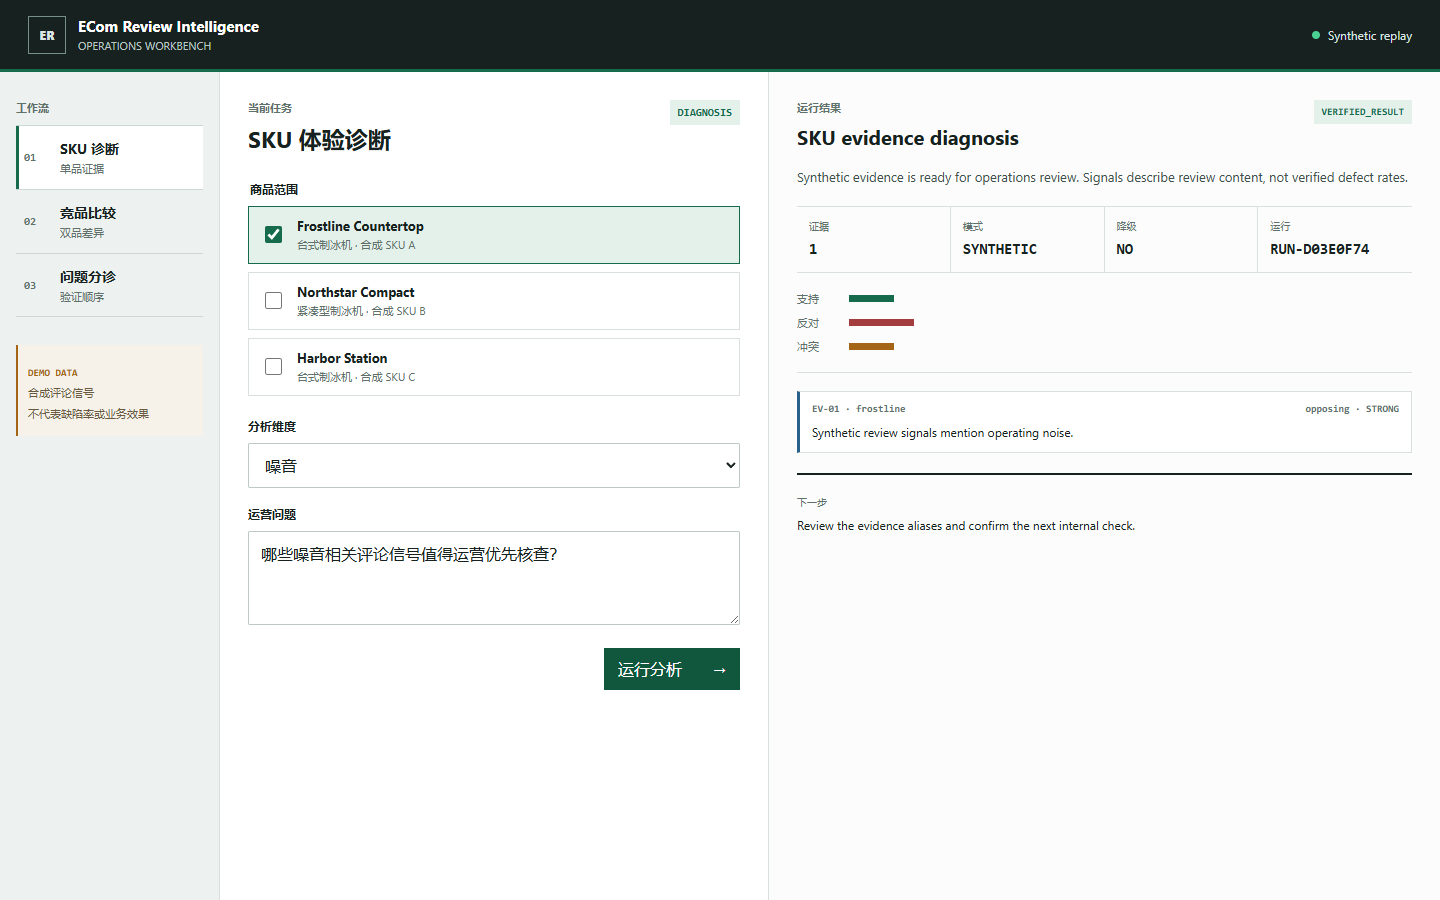
\includegraphics[width=\textwidth]{assets/p7-workbench-desktop.png}
  \caption{P7 synthetic 工作台电脑网页端。左侧选择任务，中间填写商品与问题，右侧查看状态、聚合信号、证据卡和下一步。截图只说明受控流程，不证明真人业务效果。}
  \label{fig:p7-desktop-integrated}
\end{figure}

左侧是任务导航，中间是表单，右侧是结果区。页面顶部会显示 synthetic 或 local，避免把演示数据误认为真实业务输出。

\subsection{3. 先学会看三个任务}

\textbf{SKU 体验诊断：}选择一个商品和一个维度，运行后先看状态，再看支持、反对和冲突信号，最后看优先核查项与匿名证据卡。

\textbf{竞品比较：}选择两个商品并使用同一维度，比较两边的聚合证据；结果不是购买推荐，也不是缺陷率。

\textbf{运营问题分流：}提交一个运营问题和允许比较的商品范围，结果帮助判断下一步由产品、客服或内容团队核实，不自动执行外部动作。

\subsection{4. 处理歧义并恢复}

标题命中多个候选时，状态变为 \texttt{NEEDS\_CLARIFICATION}。用户从已授权候选中选择后继续；服务用 P6 的 \texttt{checkpoint} 恢复原任务，不重新规划，也不能选择候选集合之外的商品。

\subsection{5. 读懂结果状态}

\begin{longtable}{>{\raggedright\arraybackslash}p{0.28\textwidth}>{\raggedright\arraybackslash}p{0.58\textwidth}}
\toprule
状态 & 先这样理解 \\
\midrule
\texttt{VERIFIED\_RESULT} & 当前结果通过本地规则、工具范围、Verifier 和引用门；是否行动仍由运营人员判断。 \\
\texttt{NEEDS\_CLARIFICATION} & 商品有歧义，需要在授权候选中选择，不代表程序故障。 \\
\texttt{DEGRADED\_SAFE\_RESULT} & 证据不足或检查未满足，系统给出受限结果，不补写结论。 \\
\texttt{FAILED} & 请求没有安全完成，应查看固定错误码和运行环境。 \\
\bottomrule
\end{longtable}

supporting、opposing、conflicting 是评论信号的聚合方向，不是缺陷率；evidence count 是本次允许使用的证据数量，不代表市场占比；优先核查项是下一步建议，不是自动决策。

\subsection{6. 何时使用 local 模式}

只有本地证据库、数据来路和 P6 回归均通过后，才运行：

\begin{lstlisting}
.\.venv\Scripts\python.exe scripts/run_phase7_local_regression.py --project-root .
.\.venv\Scripts\python.exe scripts/run_phase7_workbench.py --mode local --acknowledge-local-data --project-root . --port 8765
\end{lstlisting}

local 模式仍只允许浏览器看到聚合 DTO。公开截图和手册不能展示本地商品键、evidence id、路径或评论原文。

\section{问题、修复与验证}

问题包括 Host 和绝对路径扫描遗漏、旧 PASS 在失败后还存活、local 回归身份不足、工作台绕过 P6 Trace，以及自动化代替真人试用。修复包括闭集 Host/DTO、失败前失效旧工件、结构化 local 回执和真实浏览器入口验证；目标运营用户试用仍作为缺口保留，不能用开发者测试冒充。

\section{阶段产出与验收边界}

已完成的工程产出包括电脑网页端、typed API、synthetic 与受控 local adapter、电脑端截图、浏览器验证和公开聚合报告\filelink{docs/reports/phase-7-workbench-validation.md}。真人试用模板位于\filelink{docs/templates/p7-user-trial-record.md}。

P7 当前状态是 \texttt{IN\_PROGRESS}，即 \statusprogress。只有目标运营用户按模板完成任务、记录时间、证据复核和问题，才可以讨论易用性与业务价值。

\section{怎样进入下一阶段}

下一步是让真实目标用户分别完成手工流程和工作台流程，比较完成时间、错误、证据复核和主观负担，再决定权限、多人协作、监控和在线部署是否值得投入。

\section{面试怎么讲}

\begin{interviewbox}
“P7 不是给 CLI 套网页。我先定义浏览器公开 DTO，再把 synthetic 与显式 local adapter 分开，local 路径复用 P6 流程、工具和 Verifier。浏览器自动化和本地回归证明了工程接线，但目标运营用户结构化试用还没有完成，所以我不会声称已经节省工时或上线生产。”
\end{interviewbox}

\textbf{掌握标准：}能在电脑网页端完成三个任务，解释四种状态、公开 DTO 与内部 state 的边界，并准确说出 P7 为什么仍是 \texttt{IN\_PROGRESS}。

\chapter{全项目问题、修复与可迁移经验}

\begin{beginnerbox}
P0--P7 已在对应阶段解释各自的开发过程。本章不再重讲阶段，而是把跨阶段反复出现的错误前提整理成可迁移经验。一个 PASS 只有在案例、入口、指标、阻断门和代码身份都明确时才有意义。

如果你是第一次学习，可以先跳过本章。先把 P0--P7 的主线读懂，再回来把这里的失败案例当作“为什么要这样设计”的答案。
\end{beginnerbox}

\section{为什么需要分层评测}

本项目的数据、检索、Agent 和界面承担不同责任，不能用一个指标覆盖全部层次。

\begin{longtable}{p{0.12\textwidth}p{0.30\textwidth}p{0.26\textwidth}p{0.20\textwidth}}
\toprule
层次 & 主要问题 & 可以证明 & 不能证明 \\
\midrule
P1--P4 & 输入、合同、证据库是否一致 & 快照、lineage、精确关联和引用可重算 & 现实商品质量 \\
P5 & 检索是否返回预期证据 & 冻结 silver 案例内的召回、引用和无答案行为 & 人工 gold 相关性或业务效果 \\
P6 offline & Agent 图和失败分支是否稳定 & 路由、澄清、工具、引用、攻击和降级的工程行为 & 当前真实供应商可用性 \\
P6 live & 真实 DeepSeek 是否遵守当前协议 & 冻结案例和当前版本下的有界真实调用行为 & 开放输入可靠性和生产 SLA \\
P7 browser/local & 界面和 P6 接线能否受控运行 & 三工作流、恢复、公开 DTO、视口和本地接线 & 真人采纳、工时节省和决策改善 \\
\bottomrule
\end{longtable}

\section{P5：负结果同样有价值}

P5 使用预冻结 silver 案例比较简单词法基线与 FTS5/BM25。结果没有证明 BM25 在当前小范围和标签口径下更好，因此项目没有为了“技术看起来更高级”而强行增加向量数据库或复杂检索。

这项结论必须带两个边界：

\begin{enumerate}
  \item silver 期望证据部分来自同一词法口径，存在循环偏向；
  \item 冻结案例适合回归，不等于人工标注的独立 relevance 数据集。
\end{enumerate}

\begin{inferencebox}
基于当前证据，继续采用较简单检索是合理工程选择；但不能下结论说 BM25 或向量检索普遍无效。若后续建立独立人工相关性集，技术选择应重新比较。
\end{inferencebox}

\section{P6 offline：怎样防止“假通过”}

离线评测覆盖正常诊断、比较、分流、澄清、真实无答案、提示注入、越权工具、伪造标识、供应商失败和预算限制。早期实现曾出现过几类 false PASS 风险：

\begin{itemize}
  \item 根据场景名称推断“攻击已被阻止”，而不是检查真实输出；
  \item 期望引用为空时，实际也为空，从而形成引用完整性的真空通过；
  \item 无答案案例没有回真实 store 验证；
  \item 测试只验证注入对象，没有走真实编译图或真实 CLI；
  \item 失败重跑后旧的公开 PASS 仍可能存在。
\end{itemize}

修复后，评测要求 expected、tool 和 rendered 三组引用严格相等，响应中的引用逐一回本地库验证；有答案案例必须有非空真实证据；每一项状态、工作流、澄清和安全预期都是阻断门；公开摘要与报告成对发布，失败则旧 PASS 失效。

\begin{factbox}
当前公开 offline 报告记录 30 个冻结案例的阻断门通过。它证明当前冻结范围内的工程行为，不证明回答达到人工 gold 质量，也不证明 DeepSeek 随时可用。
\end{factbox}

\section{P6 live：真实模型为什么仍需本地校验}

真实 DeepSeek 接入暴露了两个递进问题。

\subsection{问题一：JSON 合法不等于业务草稿合法}

首次兼容性 smoke 中，模型可以返回可解析 JSON，但结构不是系统要求的业务草稿。修复是使用强制 tool call，让供应商按 \texttt{submit\_agent\_draft} 的 schema 提交结构化结果。

\subsection{问题二：结构合法不等于字段获得授权}

即使 schema 通过，模型仍可能改写证据卡的极性、强度或别名。补充 prompt 并不能形成可靠边界，因为 prompt 只是要求，不是执行控制。

最终方案分为两层：

\begin{enumerate}
  \item 根据本次安全证据卡动态收窄允许值，减少模型可提交空间；
  \item 本地 Verifier 逐字段核对 workflow、商品别名、aspect、卡片别名、极性、强度和引用；不一致时只允许一次修复，再失败则确定性降级。
\end{enumerate}

\begin{beginnerbox}
Structured Output 回答“格式能不能解析”；Verifier 回答“字段是不是来自这次任务授权的证据”。两者不能互相替代。
\end{beginnerbox}

\section{15 乘 2 gate 应该怎样解释}

真实模型 gate 从冻结案例中选择 15 项，每项独立运行两次。完整发布要求恰好形成 30 个独立结果，供应商记录与 HTTP 尝试对齐，任何单案例失败、重复 run/thread 或不完整重复都会阻断。

当前报告记录 26 次验证结果和 4 次预期证据不足降级，状态与引用预期全部通过，未记录越权工具、成功注入、伪造标识或公开泄漏。

\begin{boundarybox}
这不是统计显著实验，也不是模型质量排行榜。它不覆盖未来模型版本、任意用户输入、网络波动、并发、长期成本或生产运维，因此不能写成“准确率百分之百”“生产稳定”或“达到 SLA”。
\end{boundarybox}

\section{安全指标怎样避免自我证明}

安全评测必须观察真实行为，而不能由测试场景名称直接生成结论。

\begin{itemize}
  \item \textbf{提示注入：}检查攻击文本是否改变了受控 workflow、商品范围、工具或引用；
  \item \textbf{越权工具：}检查实际执行工具是否超出 router 的唯一授权；
  \item \textbf{伪造标识：}从响应提取商品、证据、卡片和运行期别名，与当前授权集合做差集；
  \item \textbf{公开泄漏：}递归扫描公开摘要、报告和响应中的禁止键和值形状；
  \item \textbf{无答案：}要求 tool 和 rendered 都没有引用，并返回明确安全降级；
  \item \textbf{预算：}模型调用、工具执行和修复次数必须在单调 ledger 内。
\end{itemize}

模型“说自己没有越权”不算证据。必须由本地执行记录、集合比较和回库校验产生指标。

\section{Trace：可观察性与隐私的平衡}

本项目采用双轨 Trace：

\begin{itemize}
  \item 本地敏感 Trace 记录调试所需状态，保持 ignored，不进入公开仓库；
  \item 公开 Trace 只保留闭集、聚合、安全字段，并经过 serializer 和值扫描。
\end{itemize}

P7 曾出现 no-op trace writer 被标为 \texttt{trace\_written=True} 的假阳性。修复后，写入成功必须对应真实目标和结果；公开 trace 继续遵守 P6 schema。Trace 证明路径和状态发生过，不证明内容现实正确。

\section{失败案例一：手工数据下载与证据边界}

\textbf{现象：}自动下载受环境限制，最终由用户手工取得文件。\par
\textbf{错误前提：}文件存在就等于获得了完整官方下载证据。\par
\textbf{根因：}手工传输缺少浏览器 HTTP 回执或官方 checksum。\par
\textbf{处理：}对本地文件做大小、gzip 完整性和本地哈希校验，并在报告中降低结论强度。\par
\textbf{面试要点：}我区分“本地文件完整”和“官方端到端传输已独立证明”，没有补造来源证据。

\section{失败案例二：算法推荐与业务选择冲突}

\textbf{现象：}P2 算法候选与最终 Ice Makers MVP 选择不完全一致。\par
\textbf{错误做法：}为了让结果看起来一致，事后调整权重。\par
\textbf{处理：}保留算法推荐，单独记录人工业务 override 和理由。\par
\textbf{学习：}数据分析负责提供证据，产品决策还要考虑求职展示、范围、时间和可解释性。

\section{失败案例三：Windows 文件句柄阻止原子替换}

\textbf{现象：}P4 构建临时 SQLite 后，Windows 因仍有连接或句柄而拒绝替换。\par
\textbf{根因：}验证逻辑仍持有文件连接；Unix 上不明显的句柄生命周期在 Windows 上成为阻断。\par
\textbf{修复：}把构建、关闭、复核和原子替换顺序显式化，失败时不覆盖旧的有效库。\par
\textbf{面试要点：}原子发布不是一个函数名，而是临时产物、完整校验、句柄释放和最终替换共同形成的行为。

\section{失败案例四：恢复流程只在假对象中通过}

\textbf{现象：}早期 clarification/resume 测试证明了注入对象，却没有证明真实 SQLite checkpoint 关闭重开后可恢复。\par
\textbf{修复：}改用不透明 UUID4 token，增加真实图、真实 store、关闭重开、跨线程隔离、错误 token 和入口级两次调用测试。\par
\textbf{学习：}单元测试可以证明局部逻辑，真实入口测试才证明组件接线。

\section{失败案例五：公开 PASS 与代码身份脱节}

\textbf{现象：}旧版本评测只记录 Git revision，工作树修改或入口脚本变化可能没有进入身份。\par
\textbf{修复：}同时记录源码摘要、dirty 状态、数据快照、合同和配置身份；私有明细由完成审计重新聚合，公开报告必须等于固定 renderer。\par
\textbf{学习：}一个 PASS 必须绑定“什么数据、什么代码、什么配置、什么案例”，否则只是无上下文标签。

\section{失败案例六：P7 工程 PASS 不能代替真人试用}

浏览器自动化可以验证元素关系、溢出、网络错误、安全响应和截图，但它不会像运营人员一样判断证据是否有用。开发者完成 synthetic 任务也不是目标用户证据。

因此 P7 状态保持 \statusprogress。真正的关闭条件是目标运营角色完成结构化试用，并记录手工基线、工作台结果、引用复核、采纳/修改/拒绝和失败原因。

\section{遇到失败时的通用分析模板}

\begin{enumerate}
  \item \textbf{现象：}只描述观察到的输出和入口；
  \item \textbf{错误前提：}指出原先把什么当成了证明；
  \item \textbf{根因：}定位到合同、数据、状态、权限、供应商或发布边界；
  \item \textbf{最小修复：}不扩大范围，只关闭当前可重现缺口；
  \item \textbf{反例测试：}先让旧实现失败，再实现修复；
  \item \textbf{真实入口验证：}避免只在 mock 或 helper 中通过；
  \item \textbf{结论边界：}写清修复证明什么，仍不能证明什么。
\end{enumerate}

\begin{interviewbox}
回答 Bad Case 时不要只说“最后修好了”。更好的结构是：“我一开始把 A 误当成 B；独立审查用这个反例证明会假通过；我先写失败测试，再把校验移到真实入口；现在能证明 C，但 D 仍需用户或生产证据。”
\end{interviewbox}

\section{证据指针}

评测结果和边界可追溯到 \filelink{docs/reports/phase-5-retrieval-evaluation.md}、\filelink{docs/reports/phase-6-offline-agent-evaluation.md}、\filelink{docs/reports/phase-6-agent-evaluation.md}、\filelink{docs/reports/phase-7-workbench-validation.md} 与 \filelink{docs/interview-casebook.md}。

\chapter{简历表达与面试复盘}

\begin{beginnerbox}
简历不是把仓库里的技术名词全部塞进去，而是用少量可证明的句子，让面试官知道：你为什么做、解决谁的问题、你负责什么、系统怎样工作、证据是什么、边界在哪里。只有自己能解释、复现和修改的内容，才适合写成“我设计”或“我实现”。

学习时先不要背整段答案。先用自己的话说清楚每个阶段解决的业务问题，再把本章的回答模板当作整理表达的工具。
\end{beginnerbox}

\section{先确定项目的一句话定位}

推荐项目名：

\begin{quote}
ECom Review Intelligence Agent：面向品牌方产品/类目运营的评论证据决策原型
\end{quote}

一句话介绍：

\begin{quote}
我围绕 SKU 诊断、竞品比较和问题分诊，构建了一个由本地证据工具掌握事实与执行权、DeepSeek 负责受约束规划和表达、Verifier 核对业务字段与引用的 LangGraph Agent。
\end{quote}

这句话比“做了一个电商 RAG 聊天机器人”更准确，因为项目包含数据合同、商品授权、确定性工具、澄清恢复、逐字段验证、评测和安全发布，而不是只有检索与生成。

\section{为什么做这个项目}

面试时可以分三层回答：

\begin{enumerate}
  \item \textbf{个人背景：}我在运营中心实习，也关注广州电商和 AI 应用岗位，希望项目能同时体现业务理解与工程能力；
  \item \textbf{业务问题：}运营阅读大量评论后，仍需要把问题信号整理成能回到证据的单品诊断、竞品比较和跨团队分诊；
  \item \textbf{技术问题：}如果只让模型自由总结，商品范围、引用、工具权限和失败状态都难以审计，因此我把事实、执行权和校验留在本地代码。
\end{enumerate}

\begin{boundarybox}
广州和运营实习是选题动机，不是完整市场证明。可以说“这个方向与我的目标岗位和经历匹配”，不能说“广州所有电商公司都需要”或“市场已经验证付费意愿”。
\end{boundarybox}

\section{通用简历版本}

可根据版面选三到四条：

\begin{itemize}
  \item 面向品牌方产品/类目运营，定义 SKU 诊断、竞品比较和问题分诊三条评论证据工作流，将效率、决策支持与治理价值假设和已验证工程结果分开。
  \item 从冻结数据快照、VOC 证据合同到 SQLite/FTS5 本地证据库建立可重算 lineage，并用稳定本地引用、精确商品关联和公开边界支持可复核分析。
  \item 构建受约束 LangGraph 单 Agent，结合严格 Structured Output、本地确定性工具、一次澄清恢复、checkpoint、请求预算、安全证据卡、逐字段 Verifier 和失败关闭。
  \item 完成 30 个冻结离线 Agent 案例及真实 DeepSeek 15 乘 2 有界评估，并将 Agent 封装为 loopback-only typed API 与桌面/移动运营工作台；P7 真人运营试用仍待完成。
\end{itemize}

\section{按岗位调整重点}

\subsection{AI 产品或数据产品岗位}

强调：为什么选这个问题、主用户是谁、三工作流如何从需求到指标、为什么控制 MVP、怎样区分价值假设与工程事实、下一步怎样做用户验证。

可替换 bullet：

\begin{quote}
设计“原流程与工作台同任务比较”的 P7 用户试用方案，计划记录首次有效证据、引用复核、采纳/修改/拒绝和失败原因；在目标用户试用前不宣称节省工时或改善决策。
\end{quote}

\subsection{AI 应用或 Agent 岗位}

强调：严格 DTO、tool/authority 分离、LangGraph 状态、interrupt/resume、checkpoint、Verifier、fake/replay/live、离线与真实模型 gate、公开/私有 Trace 和失败原子发布。

可替换 bullet：

\begin{quote}
修复真实模型“JSON 合法但业务字段未授权”的问题，通过动态收窄 schema 与本地逐字段 Verifier 核对 workflow、别名、极性、强度和引用，失败只修复一次后确定性降级。
\end{quote}

\subsection{电商运营或 VOC 岗位}

强调：评论证据怎样支持单品体验问题整理、竞品同维度比较、质量/客服协同和下一步核查；避免大段讲框架内部实现。

可替换 bullet：

\begin{quote}
围绕噪声、可靠性、清洁维护等八类 VOC 维度，将评论问题信号整理为可追溯证据卡和进一步核查建议，明确不把评论频次外推为缺陷率、销量损失或因果结论。
\end{quote}

\section{30 秒介绍}

\begin{quote}
我做的是一个面向品牌方产品和类目运营的评论证据 Agent，支持 SKU 诊断、竞品比较和问题分诊。它不是让模型直接掌握事实，而是由本地工具取证，模型做受约束规划和表达，Verifier 再核对引用和业务规则。P0 到 P6 已通过，P7 的 synthetic 桌面/移动验证和 P6-backed 本地三工作流回归也已通过；但目标运营用户尚未试用，所以我不宣称已经产生业务效率或降本增效。
\end{quote}

\section{1 分钟介绍}

\begin{quote}
这个项目来自我的运营中心实习和广州电商求职方向。我发现普通评论摘要很难回答“结论能否回到证据”和“模型有没有越权”，所以我把项目定义成 B 端内部决策支持原型，而不是消费者聊天助手。

数据层先冻结来源、品类范围和八类 VOC 合同，再用 SQLite/FTS5 建本地证据库。Agent 层用 LangGraph 管理诊断、比较、分流和一次澄清恢复；外部 DeepSeek 只看到匿名安全卡，本地 resolver、router、tool ledger 和 Verifier 分别掌握商品、工具、次数和事实授权。

验证上，我保留了检索负结果和 Bad Case，完成离线 30 案例与真实模型 15 乘 2 有界 gate。P7 工作台工程路径已验证，但真人运营试用仍未完成，所以当前结论是“工程闭环可复核”，不是“业务效果已证明”。
\end{quote}

\section{3 分钟介绍}

\begin{quote}
我希望这个项目同时能回答业务和技术两个问题。业务上，品牌方产品或类目运营需要从大量评论中整理单品问题、竞品差异和跨团队核查优先级；技术上，直接让大模型总结会把商品范围、工具权限、引用和失败状态都交给一个概率模型，难以审计。

因此我先没有做 Agent。P0 和 P1 验证数据源并冻结快照，P2 通过流式审计选择 Ice Makers 作为两个月 MVP，P3 冻结 VOC、极性、强度和引用合同，P4 建 SQLite/FTS5 确定性证据库，P5 用冻结 silver 案例比较检索基线并保留 BM25 没有独立胜出的负结果。这样 P6 的模型只能消费已经定义的证据，而不能临时改变口径。

P6 使用 LangGraph 管理状态和分支。输入先经 Pydantic，模型提交受约束计划，本地 resolver 决定商品，router 只授权一个业务工具，ledger 限制执行次数。工具返回后，本地代码把结果变成匿名安全卡，DeepSeek 提交结构化草稿，Verifier 再逐字段核对 workflow、商品别名、aspect、卡片、极性、强度和引用。标题歧义时 interrupt 并通过 UUID4 token resume；模型失败、证据不足或二次拒绝时确定性降级。

我遇到过两个关键问题：一是离线评测曾可能零引用真空通过，后来改成 expected、tool、rendered 引用三方相等并逐一回库；二是真实 DeepSeek 即使返回合法 JSON，也会改写业务字段，因此增加动态 schema 与本地 Verifier。最后完成离线 30 案例、真实模型 15 个案例各两次的有界 gate 和完成审计。

P7 把这张图封装成 loopback-only typed API 和运营工作台，synthetic 浏览器与本地三工作流接线已经验证。现在最重要的下一步不是再加框架，而是让目标运营用户完成同任务的手工基线和工作台试用，记录首次有效证据、引用复核、采纳和失败原因。只有拿到这些证据后，才能讨论是否真正节省时间或改善决策。
\end{quote}

\section{高频业务问题}

\subsection{Q1：项目的业务价值到底是什么？}

\textbf{回答框架：}当前已实现的是把评论整理为可追溯的诊断、比较和分诊证据，可能减少重复筛选并改善跨团队沟通；工程治理价值已经验证，效率和决策改善仍待目标用户试用。不要直接说“降本增效”。

\subsection{Q2：为什么主要面向 B 端，不直接做消费者助手？}

\textbf{回答框架：}我的经历和目标岗位更接近运营；B 端任务需要证据、协作和审计，能体现产品与工程闭环。底层能力未来可支持 C 端，但当前 MVP 不做推荐、价格和库存决策。

\subsection{Q3：运营为什么不用 Excel 或 BI？}

\textbf{回答框架：}Excel/BI 很适合结构化指标，本项目补的是评论文本到证据卡、受控工作流和可复核自然语言之间的环节。是否值得替代现有流程仍需要用户试验，不能假设 Agent 一定更好。

\subsection{Q4：怎样验证业务价值？}

\textbf{回答框架：}对同一任务先做原流程，再做工作台流程，记录完成时间、首次有效证据、引用复核、采纳/修改/拒绝和失败原因。单个用户只能形成定性观察，扩大结论需要更多角色和任务。

\section{高频技术问题}

\subsection{Q5：为什么这不是普通 RAG？}

检索只是其中一层。系统还包含商品授权、三工作流、澄清恢复、工具 ledger、逐字段 Verifier、请求预算、双轨 Trace、离线/live gate 和失败原子发布。

\subsection{Q6：为什么用 LangGraph？不用行不行？}

固定脚本也能实现简单主路径。选择 LangGraph 是因为项目有澄清暂停、恢复、一次修复、确定性降级和 checkpoint，需要把节点和状态显式化。LangGraph 负责编排，不替代业务校验或安全策略。

\subsection{Q7：Structured Output 已经有 schema，为什么还要 Verifier？}

schema 只能保证字段与类型可以解析，不能保证这些值来自本次授权证据。真实模型曾返回结构合法但极性或强度未授权的结果，所以本地 Verifier 必须逐字段比较。

\subsection{Q8：怎样防止幻觉？}

不承诺消灭幻觉。调用前只发送匿名安全卡；模型无数据库和任意工具权限；生成后逐字段校验，引用三方相等并回库；失败只修复一次，再失败则安全降级。

\subsection{Q9：为什么不用向量数据库？}

P5 的当前冻结案例没有证明复杂检索的独立收益，而且 silver 集有词法循环偏向。应先建立人工 relevance 数据集，再决定是否引入向量检索，而不是为简历堆技术。

\subsection{Q10：Fake、Replay 和 Live 有什么区别？}

fake 用于程序内故障注入，replay 用于冻结复现，live 才验证真实供应商协议和行为。任何一种模式通过，都不能替代另外两种想证明的内容。

\subsection{Q11：15 乘 2 能证明生产可靠性吗？}

不能。它证明当前代码、配置、冻结案例和当前供应商版本下的有界行为，不覆盖开放输入、并发、长期网络波动、未来模型版本和生产 SLA。

\subsection{Q12：checkpoint 里存了什么？}

存可序列化的 Agent 状态和预算，不存 live client 或不可序列化对象。恢复时重新注入运行时依赖，token 必须属于原线程且预算只能单调增加。

\section{失败案例追问}

\subsection{Q13：最有价值的失败是什么？}

可以回答离线 false PASS：早期引用可能在空集合上真空通过，安全计数也可能由场景推导。我先写反例测试，再要求 expected/tool/rendered 三方相等、回真实库验证，并让每个业务与安全预期成为阻断门。这个案例体现了我对“测试通过能证明什么”的重新理解。

\subsection{Q14：真实 API 接入最难的地方是什么？}

不是把 HTTP 请求发出去，而是区分协议格式和业务授权。JSON mode 解决可解析问题，强制 tool call 解决草稿结构，动态 schema 和本地 Verifier 才解决当前证据授权。

\subsection{Q15：P7 为什么还没有完成？}

工程自动化、桌面移动视口和 P6-backed 本地接线已经验证，但验收定义还要求目标运营用户的结构化试用。开发者自动化不能替代用户是否理解、采纳和完成任务的证据。

\section{压力问题和诚实回答}

\subsection{“你是不是用 AI 写的？”}

如实说明 AI 用于生成、审查、测试建议和文档整理。个人贡献用四件事界定：能否解释设计取舍、能否从干净环境复现、能否在反例下修改、能否对结论边界负责。不要把 AI 生成的每行代码都说成纯手写。

\subsection{“这个项目真的有人用吗？”}

当前没有目标运营用户完成正式结构化试用。可以展示 synthetic 和 local 工程证据，但不能把自己或自动化浏览器称为真实用户。下一步试用计划已经定义。

\subsection{“业务指标是多少？”}

当前没有可靠的工时节省、采纳率或决策质量指标。开发者时延和测试通过数不是业务指标。若面试官需要，可以说明准备怎样测，而不是现场编造数字。

\subsection{“你不会的问题怎么办？”}

先说明目前能确认的证据，再指出缺少什么信息。例如：“我目前没有多租户和生产并发证据，所以不能判断部署规模；我会先定义流量、隔离和 SLA，再做容量与故障测试。”证据不足不等于结论错误，但不能装成已确认。

\section{当前系统边界清单}

面试中应主动说明当前不是成熟企业 SaaS，仍缺：

\begin{itemize}
  \item 多租户、RBAC、企业身份和团队任务流；
  \item 企业数据连接器、持续数据更新和运营后台；
  \item 生产监控、告警、并发、成本治理和 SLA；
  \item 人工 gold 相关性集和更开放的质量评估；
  \item 多名目标运营用户的真实任务与业务效果证据。
\end{itemize}

主动说边界不会削弱项目，反而说明你知道原型、工程验证、用户验证和生产系统之间的区别。

\section{面试前自测}

\begin{enumerate}
  \item 能否不看文档画出一次完整请求的主路径和三条分支？
  \item 能否用自己的话解释为什么模型没有商品和工具执行权？
  \item 能否运行 synthetic 工作台并解释每个状态？
  \item 能否复现一个验证失败或证据不足分支？
  \item 能否说出 P5、P6 offline、P6 live 和 P7 各自能证明什么？
  \item 能否讲清一个真实 Bad Case 的 RED、修复和 GREEN？
  \item 能否在不夸大结果的情况下回答项目价值？
  \item 能否明确 P7 为什么仍为 \statusprogress？
\end{enumerate}

如果其中任何一项只能背诵，先回到对应章节做练习，再把它写进简历。

\section{证据指针}

本章的详细案例和问答依据 \filelink{docs/interview-casebook.md}，阶段状态以 \filelink{docs/master-plan.md} 和 \filelink{docs/current-stage-status.md} 为准。具体评测结论应回到 P5、P6 与 P7 的公开报告，不使用可能过期的口头数字替代同版本证据。

\chapter{复现、Overleaf 与后续路线}

\begin{beginnerbox}
本章解决三个实际问题：怎样运行项目、怎样配置可选的 DeepSeek Key、怎样把这套 LaTeX 工程上传到 Overleaf 并得到 PDF。三者不是同一件事：阅读和编译手册不需要 API；默认工作台也不调用 DeepSeek。

第一次复现建议只做“阅读手册”和“编译手册”两层：先确认自己能读懂主线，再尝试修改一小段文字并在 Overleaf 重新编译。synthetic 工作台、本地回归和真实模型 gate 属于后续练习。
\end{beginnerbox}

\section{先选择你真正需要的复现层级}

\begin{longtable}{p{0.18\textwidth}p{0.30\textwidth}p{0.38\textwidth}}
\toprule
层级 & 适合做什么 & 需要什么 \\
\midrule
阅读手册 & 学习项目、准备简历与面试 & PDF 阅读器即可 \\
编译手册 & 修改文字、替换截图、学习 LaTeX & Overleaf 或本地 Tectonic/XeLaTeX \\
synthetic 工作台 & 演示界面和三个运营流程 & Python 环境；不需要原始数据和 API Key \\
本地受控回归 & 验证 P7 到 P6 图和 SQLite 工具的接线 & 已有本地处理数据；需要显式确认 \\
真实模型 gate & 验证当前 DeepSeek 协议和冻结案例 & API Key、联网、预算和显式确认 \\
\bottomrule
\end{longtable}

\begin{boundarybox}
能运行上一层，不自动证明下一层。例如：Overleaf 编译成功只证明文档工程完整；synthetic 页面能操作只证明受控演示流程；真实模型 gate 通过也不等于生产 SLA 或真实业务效果。
\end{boundarybox}

\section{Windows 上建立 Python 环境}

打开 PowerShell，进入仓库根目录后执行：

\begin{lstlisting}[language={}]
python -m venv .venv
.\.venv\Scripts\python.exe -m pip install -e ".[dev]"
.\.venv\Scripts\python.exe -m pytest
.\.venv\Scripts\python.exe -m ruff check .
\end{lstlisting}

如果看到命令行左侧出现 PowerShell 提示符，不需要先激活虚拟环境，因为命令已经直接指定了虚拟环境内的 Python。这样比依赖当前窗口是否激活更容易复现。

\section{运行默认 P7 工作台}

先做不启动服务的配置检查：

\begin{lstlisting}[language={}]
.\.venv\Scripts\python.exe scripts\run_phase7_workbench.py --check
\end{lstlisting}

再启动默认 synthetic 模式：

\begin{lstlisting}[language={}]
.\.venv\Scripts\python.exe scripts\run_phase7_workbench.py --port 8765
\end{lstlisting}

浏览器访问 \url{http://127.0.0.1:8765}。synthetic 是“确定性演示数据”，用于验证界面和流程；它不读取 DeepSeek Key，不读取原始评论，也不展示本地商品或证据标识。

结束服务时，回到启动服务的 PowerShell 窗口，按 \texttt{Ctrl+C}。如果页面打不开，依次检查：命令是否仍在运行、端口是否被占用、浏览器地址是否为 loopback 地址、终端是否出现固定错误信息。

\section{DeepSeek Key：什么时候才需要}

\subsection{不需要 Key 的情况}

下列工作都不需要 Key：阅读或编译手册、运行单元测试、运行默认 synthetic 工作台、阅读已经提交的聚合评测报告。

\subsection{需要 Key 的情况}

只有你明确运行真实 DeepSeek smoke 或 live evaluation 时才需要。Key 不应写进 Python、LaTeX、Markdown、命令参数、截图、日志、\texttt{.env} 或 Git 提交。

\subsection{推荐的 Windows 用户环境变量方法}

在 PowerShell 中运行下面的命令，将尖括号内容替换为自己的 Key。该命令会把值保存为当前 Windows 用户环境变量；关闭并重新打开 PowerShell 后才会自然进入新进程。

\begin{lstlisting}[language={}]
[Environment]::SetEnvironmentVariable(
  "DEEPSEEK_API_KEY",
  "<your-key>",
  "User"
)
\end{lstlisting}

不要把真实值复制进手册或提交记录。配置完成后，关闭当前 PowerShell，重新打开一个窗口，再用布尔值检查存在性：

\begin{lstlisting}[language={}]
[bool]$env:DEEPSEEK_API_KEY
\end{lstlisting}

返回 \texttt{True} 表示当前进程看到了变量；不要使用会把完整值打印到屏幕的命令。若返回 \texttt{False}，先检查是否重新打开了 PowerShell，再检查用户环境变量名称拼写。PowerShell 与传统 CMD 都能运行项目，但本项目文档和命令以 PowerShell 为准。

\subsection{运行有界 live gate}

先只运行一个兼容性 smoke：

\begin{lstlisting}[language={}]
.\.venv\Scripts\python.exe scripts\run_phase6_live_evaluation.py \
  --project-root . --case-limit 1 --acknowledge-live-api
\end{lstlisting}

只有 smoke 成功、预算允许且明确理解会产生 API 调用时，才执行冻结案例的两次重复 gate：

\begin{lstlisting}[language={}]
.\.venv\Scripts\python.exe scripts\run_phase6_live_evaluation.py \
  --project-root . --repetitions 2 --acknowledge-live-api
\end{lstlisting}

\begin{boundarybox}
单案例 smoke 不发布 PASS。完整 gate 也只证明当前代码、当前配置和冻结案例下的有界行为。模型版本、网络和供应商策略可能变化，因此旧结果不能替代未来重跑。
\end{boundarybox}

\section{把 LaTeX 工程上传到 Overleaf}

\subsection{第一步：准备 ZIP}

只压缩 \filelink{docs/project-handbook/} 目录中的内容。ZIP 根目录打开后应直接看到 \filelink{main.tex}、\filelink{preamble.tex}、\filelink{chapters/} 和 \filelink{assets/}，不要多套一层本机绝对目录。

\subsection{第二步：创建项目}

登录 Overleaf，选择“New Project”中的“Upload Project”，上传 ZIP。上传完成后，在左侧文件树确认九个章节和两张 PNG 截图都存在。

\subsection{第三步：选择编译器}

打开项目菜单，将 Compiler 设为 \textbf{XeLaTeX}，将 Main document 设为 \filelink{main.tex}。本工程使用 \texttt{ctexbook} 和 Fandol 字体，目的是避免依赖某一台 Windows 电脑的私有中文字体。

\subsection{第四步：编译和下载}

点击 Recompile。目录和交叉引用首次可能需要多轮编译，Overleaf 会自动处理常见情况。右侧 PDF 正常显示后，使用 Download PDF 下载。

\subsection{第五步：定位常见错误}

\begin{longtable}{p{0.25\textwidth}p{0.62\textwidth}}
\toprule
现象 & 优先检查 \\
\midrule
中文乱码或字体错误 & 编译器是否误选为 pdfLaTeX；应使用 XeLaTeX \\
找不到章节 & ZIP 是否保留 \filelink{chapters/}，\texttt{main.tex} 中相对路径是否被改动 \\
找不到截图 & \filelink{assets/} 是否完整，文件名大小写是否一致 \\
百分号后文字消失 & LaTeX 中百分号是注释符号，正文百分比应正确转义 \\
下划线报错 & 普通正文中的下划线应转义或放入等宽命令 \\
表格越界 & 缩短单元格、改用跨页表，不要把整表缩到无法阅读 \\
目录页码未更新 & 再编译一次，确保交叉引用稳定 \\
\bottomrule
\end{longtable}

\section{本地编译与验证}

仓库提供固定入口：

\begin{lstlisting}[language={}]
powershell -ExecutionPolicy Bypass \
  -File scripts/build_project_handbook.ps1
.\.venv\Scripts\python.exe scripts\verify_project_handbook.py \
  --project-root .
\end{lstlisting}

最终 PDF 位于：

\begin{lstlisting}[language={}]
output/pdf/ecom-review-intelligence-project-handbook.pdf
\end{lstlisting}

构建中间文件只进入 \filelink{tmp/pdfs/project-handbook/}。验证器检查章节文本、截图嵌入、页数、编译日志和公开安全边界。文本检查不能代替视觉检查，因此最终还必须把每一页渲染为 PNG，检查重叠、裁切、乱码、黑块、空页和不可读表格。

\section{修改手册时的安全规则}

\begin{enumerate}
  \item 只写仓库相对路径，不写本机盘符路径。
  \item 不复制原始评论、真实商品标识、本地证据标识或私有岗位材料。
  \item 不写 Key 值，不把包含 Key 的终端截图放入文档。
  \item 更新阶段状态时，同时核对 canonical master plan 和当前状态页。
  \item 测试结果必须来自同一版本的实际运行，不沿用可能过期的数字。
  \item 自动化验证和真人业务验证必须分开表述。
\end{enumerate}

\section{后续路线}

当前最重要的下一步不是继续增加框架，而是完成 P7 目标运营用户的结构化试用。至少一名目标角色应对同一组任务分别完成手工基线和工作台操作，记录首次有效证据、引用复核、采纳/修改/拒绝及失败原因。

在得到真实试用证据前，可以提出“可能减少重复筛选和整理”的价值假设，但不能声称已经节省工时或改善决策。若试用显示问题不在评论检索，而在企业数据接入、团队协作或权限审批，下一阶段应优先修正产品定义，而不是继续增加 Agent 节点。

\begin{interviewbox}
复现能力本身就是面试证据。比起背诵框架名称，更有说服力的表达是：我能从干净环境启动受控模式，解释每个 gate 为什么存在，复现一个失败分支，并清楚说明哪些结论还没有真实用户证据。
\end{interviewbox}


\backmatter
\chapter*{结语}
这份手册的目标不是证明项目没有缺点，而是让每个已验证结论都能找到证据，让每个未完成事项都保持可见。
\end{document}
